\documentclass[11pt,a4paper]{report}
\usepackage[utf8]{inputenc}
\usepackage[english]{babel}
\usepackage{amsmath}
\usepackage{amsfonts}
\usepackage{amssymb}
\usepackage{amsthm}
\usepackage{mathrsfs}
\usepackage{mathtools}
\usepackage[shortlabels]{enumitem}
\usepackage{physics}
\usepackage{witharrows}
\usepackage{xifthen}
\usepackage[margin=1cm]{caption}
\usepackage{subcaption}
\usepackage{braket}
\usepackage{slashed}
\usepackage{bm}
\usepackage{geometry}
\usepackage{xcolor}
\usepackage{dsfont}
\usepackage{tensor}
\usepackage{cancel}
\usepackage{tikz}
\usepackage{tikz-cd}
\usepackage{pgfplots}
\pgfplotsset{compat=1.18}
\usepackage{fancyhdr}
\pagestyle{fancy}
\setlength{\headheight}{13.6pt}
\usepackage{biblatex} %[style=alphabetic]
\addbibresource{references.bib}
\usepackage{tocloft}
\usepackage{microtype}
\usepackage{csquotes}
\usepackage{upgreek}
\usepackage{nicematrix}
\usepackage[hidelinks]{hyperref}

\usepackage[normalem]{ulem}
\newcommand{\st}[1]{\ifmmode\text{\sout{\ensuremath{#1}}}\else\sout{#1}\fi}

\interfootnotelinepenalty=10000

\newtheorem{theorem}{Theorem}[section]
\newtheorem{proposition}[theorem]{Proposition}
\newtheorem{lemma}[theorem]{Lemma}
\newtheorem{corollary}[theorem]{Corollary}

\theoremstyle{definition}
\newtheorem{example}[theorem]{Example}
\newtheorem{definition}[theorem]{Definition}

\theoremstyle{remark}
\newtheorem*{remark}{Remark}


\DeclareMathOperator{\Vol}{Vol}
\DeclareMathOperator{\On}{O}
\renewcommand{\O}{\On}
\DeclareMathOperator{\SO}{SO}
\DeclareMathOperator{\U}{U}
\DeclareMathOperator{\SU}{SU}
\DeclareMathOperator{\id}{id}
\DeclareMathOperator{\gl}{GL}
\DeclareMathOperator{\Ad}{Ad}
\DeclareMathOperator{\ad}{ad}
\DeclareMathOperator{\Alt}{Alt}
\DeclareMathOperator{\diag}{diag}
\DeclareMathOperator{\e}{e}
\DeclareMathOperator{\im}{im}

% Footnote symbols instead of numbers
%\renewcommand{\thefootnote}{\fnsymbol{footnote}}

\newcommand{\DD}{{\rm D}}
\renewcommand{\qed}{%
	\ifmmode\tag*{$\square$}
	\else\hfill$\square$
	\fi}
\newcommand{\?}{\stackrel{?}{=}}
\newcommand{\N}{\mathbb{N}}
\newcommand{\Z}{\mathbb{Z}}
\newcommand{\R}{\mathbb{R}}
\newcommand{\RP}{\R P}
\newcommand{\C}{\mathbb{C}}
\newcommand{\F}{\mathbb{F}}
\newcommand{\T}{\mathbb{T}}
\newcommand{\Mn}[1][\C]{\mathcal{M}_n(#1)}
\newcommand{\GLn}[1][\C]{\gl_n(#1)}
\newcommand{\GL}[1][n]{\gl_{#1}(\C)}
\newcommand{\Lie}[1]{\mathcal{L}_{#1}}
\newcommand{\la}[1][g]{\mathfrak{#1}}
\newcommand{\vct}{\mathfrak{X}}
\newcommand{\Lg}{\mathscr{L}}
\newcommand{\Ac}{\mathcal{A}}
\newcommand{\Fc}{\mathcal{F}}
\newcommand{\Gc}{\mathcal{G}}
\newcommand{\Rc}{\mathcal{R}}
\newcommand{\Oc}{\mathcal{O}}
\newcommand{\Hc}{\mathcal{H}}
\newcommand{\Cinf}{C^\infty}
\newcommand{\cov}[1]{\nabla_{\!#1}}
\newcommand{\inner}[2]{\langle #1, #2 \rangle}
\newcommand{\onto}{\hookrightarrow}
\newcommand{\supto}{\supset\kern-1.7pt\to}
\newcommand{\tran}{^{\mkern-1.5mu\mathsf{T}}}
\newcommand{\herm}{^\dag}
\newcommand{\ext}[1]{\widetilde{#1}}
\newcommand{\argdot}{\makebox[1ex]{\textbf{$\cdot$}}}

\newcommand{\red}[1]{\textcolor{red}{#1}}
\newcommand{\blue}[1]{\textcolor{blue}{#1}}

\newcommand{\markedchapter}[2]{\chapter[#2]{#2%
	\chaptermark{#1}}
	\chaptermark{#1}}

\newcommand{\markedsection}[2]{\section[#2]{#2%
	\sectionmark{#1}}
	\sectionmark{#1}}
%TODO check whether shorter headings are necessary in the final report

\newcommand{\h}{\vb{h}}
\renewcommand{\k}{\vb{k}}

%\includeonly{Chapters/non-orientable}  % For generating a single chapter PDF

\begin{document}
	
\pagenumbering{roman}
\begin{titlepage}  % Suppresses page number, next page is numbered 'i' by default
	\center
	
	\textsc{\LARGE Utrecht University}\\[1.5cm]  % Main heading
	
	%------------------------------------------------
	%	Title
	%------------------------------------------------
	
	\rule{\linewidth}{0.5mm}\\[0.4cm]
	
	{\Huge\textsc{Topology of Weyl semimetals}\\[.2cm] \huge  with non-orientable Brillouin zones}\\[0.4cm] % Title
	
	\rule{\linewidth}{0.5mm}\\[.8cm]
	
	
	{\large by}\\[.8cm]
	
	
	{\LARGE Thijs \textsc{Douwes}}\\[1.1cm]
	
	
	
	{\Large \textsc{A thesis}}\\[.8cm]
	
	
	{\large Submitted to the Department of Physics}\\[.1cm]
	{\large in partial fulfilment of the requirements}\\[.1cm]
	{\large for the degree of}\\[.5cm]
	
	{\Large Master of Science}\\[.9cm]
	
	
	{\large under the joint supervision of}\\[1cm]
	
	
	\begin{minipage}{0.45\textwidth}
		\begin{flushleft}
			\large
			\textit{Project supervisor}\\
			Prof. Cristiane \textsc{de Morais Smith}\\
			\normalsize Department of Physics
		\end{flushleft}
	\end{minipage}
	~
	\begin{minipage}{0.45\textwidth}
		\begin{flushright}
			\large
			\textit{Direct supervisor}\\
			Dr. Marcus \textsc{St{\aa}lhammar}\\
			\normalsize Department of Physics
		\end{flushright}
	\end{minipage}
	
	
	\vfill\vfill\vfill  % Position the date 3/4 down the remaining page
	
	{\large October 2024}  % Use \today for current date
	
	\vfill  % Push the date up 1/4 of the remaining page
\end{titlepage}
%TODO title page
\setcounter{page}{2}  % Number next page as 'ii' instead of 'i'
	
\chapter*{Abstract}

Weyl semimetals (WSMs) are a class of 3D materials that feature point-like band crossings in momentum space. These crossings are called Weyl points, since they represent Weyl fermion-like chiral modes in the material. In a generic WSM, the so-called Nielsen–Ninomiya theorem restricts the chiralities of these Weyl points to add to zero on the momentum space unit cell—commonly referred to as the Brillouin zone. This cancellation prevents global chiral anomalies from appearing in a material.

However, recent work indicates that the Nielsen–Ninomiya theorem is circumvented when the Brillouin zone is non-orientable—a condition which can be physically realised under certain symmetries. For example, two isolated Weyl points with the same charge may appear in this scenario.

The aim of this thesis is to shed light on this and other features of non-orientable WSMs. We do this by extending an existing algebraic topology framework, which studies WSMs in terms of cohomology and homology, to the non-orientable case. This allows the physics of these systems to be studied in a more rigorous, coordinate-free setting. In particular, we are able to pinpoint the mechanism behind the circumvention of the Nielsen–Ninomiya theorem and assess its physical consequences. In addition to this, we generalise the setting to previously unstudied non-orientable Brillouin zones and other forms of orientation-reversing symmetry.

%TODO meh?
	
\tableofcontents
	
\pagenumbering{arabic}

%TODO check -ize vs. -ise in final report

\chapter{Introduction}

\section{Motivation}

\section{State-of-the-art} %TODO necessary? or merge with motivation

\section{Main question}

\section{Main results}

\section{Notational conventions}

{\color{blue}
\begin{itemize}
	\item Berry curvature factor $2\pi$ %TODO Berry curvature factor 2π
\end{itemize}
}
	
\markedchapter{Topological states}{Topological states of matter \& symmetries}

\blue{Sources: \cites{Akhmerov_online-course}{Asboth_topo-course}{Bernevig_topological-insulators}{Sato_superconductors}}

\blue{Topo phases occur in nature: \cite{Gehring_natural-TI}}

\red{Finish intro when chapter is more complete} %TODO

\section{Basic definitions}
{\color{blue}
\begin{itemize}
	\item Conducting properties of materials are understood in terms of band structure → Fermi energy. Conductance means Fermi level lies inside one of the bands. [picture]
	
	\item $N$-band system has hilbert space $\Hc\cong\C^N$, Hamiltonian represented by $N\times N$ matrix. Static system: $H\psi = E\psi$, eigenvalues are energy bands.
	
	\item Mostly interested in 2-band systems since only valence/conduction bands are relevant. Then $H$ is a $2\times 2$ Hermitian (for now) matrix. These are given by $H = h_0\mathbb{I} + \h\cdot\bm{\upsigma}$ in general ($h_0$ changes the energy of all bands but does not affect topology of band crossings) → Bloch Hamiltonian [higher dimensional systems: Clifford algebra]
	
	\item For a Bloch Hamiltonian, eigenvalues are $\pm\abs{\h}$, so conductance occurs when $\h = 0$.
	
	\item Insulating Hamiltonians are adiabatically connected if they can be continuously deformed into each other without band crossings. Insulators are considered topological if they are not adiabatically connected to a reference trivial phase; then these inhabit different regions of the phase diagram → existence of edge states (not always \cite{Bernevig_topological-insulators}, footnote)
\end{itemize}
}

\subsection{Bloch theory}
{\color{blue}
\begin{itemize}
	\item We work with crystalline materials which are composed of periodically repeating unit cells.
	
	\item In the bulk, we assume the Hamiltonian is periodic in the unit cell. This enables use of Bloch's theorem \cite{Bloch_theorem} $\psi(\vb{r}) = \e^{i\k\cdot\vb{r}}u_{\k}(\vb{r})$.
	
	\item Different values of crystal momentum may yield identical eigenstates, the set of equivalence classes is the Brillouin zone
	
	\item Brillouin zone usually has $\T^n$ topology, but internal symmetries etc. may alter this \cite{Foncesca-Vaidya_nonorientable} [other sources]
	
	\item Discuss dispersion relations
\end{itemize}
}


\section{The Su--Schrieffer--Heeger model}
{\color{blue}
	\begin{itemize}
		\item SSH is usually introduced "physics first", but we would like to work backwards in a sense, to see how bulk topology gives rise to physical properties of a system.
	\end{itemize}
}

We will take the approach of deriving the Su--Schrieffer--Heeger (SSH) model by beginning with a generic one-dimensional crystal, and introducing two topologically distinct phases in the simplest way possible.

Concretely, consider an infinite one-dimensional chain of unit cells indexed by $n\in\Z$; at this point, we make no assumptions on the internal structure of these unit cells. A boundary will be introduced later, but its relevant properties will turn out to be determined by the crystal's bulk topology. Suppose the real-space Hamiltonian of the system is periodic in the unit cells. By Bloch's theorem, two crystal momenta $k$ and $k'$ are then equivalent if they differ by an integer multiple of $2\pi$. This means that the Brillouin zone $B$ can be taken to be the interval $[-\pi,\pi]$, with the points $-\pi$ and $\pi$ identified; this space is homeomorphic to the circle $S^1$.

We might begin with a simple two-band Bloch Hamiltonian $H(k) = \h(k)\cdot\bm{\upsigma}$, with
\[
	\h: B\cong S^1\to\R^3,\quad k\mapsto\begin{pmatrix}
		h_x(k) \\ h_y(k) \\ h_z(k)
	\end{pmatrix}.
\]
Such a Hamiltonian describes a gapped phase precisely when the map $\h$ is non-zero everywhere, so that the topological classification of these phases is given by classes of maps from $S^1$ to $\R^3$ minus the origin---that is, homotopy classes of loops in $\R^3\setminus\set{0}$. However, this space has a trivial fundamental group $\pi_1\big(\R^3\setminus\set{0}\big)\cong0$, meaning that all such loops can be contracted to a point; in other words, all gapped Hamiltonians are adiabatically connected, and there are no topologically interesting phases.

This situation can be remedied by imposing a constraint on the Hamiltonian: we require that $h_z(k)=0$. Doing this effectively reduces $\h$ to a two-dimensional map:
\[
	\h: B\cong S^1\to\R^3,\quad k\mapsto\begin{pmatrix}
		h_x(k) \\ h_y(k)
	\end{pmatrix}.
\]
The gapped phases are now classified by the non-trivial fundamental group $\pi_1\big(\R^2\setminus\set{0}\big)\cong\Z$. This group is indexed by winding number: loops that wind around the origin $a\in\Z$ times cannot be deformed into those with a different winding number $b\neq a$. In particular, loops with a non-zero winding number cannot be contracted to a point, and the associated phases are considered topological. Note that imposing a constraint on the Hamiltonian has made this system rather more interesting from a topological point of view, even though it seems like it has been simplified. Once we move to the physical picture, we will see that this restriction corresponds to imposing a certain symmetry on the system.

Let us now choose a more specific Hamiltonian to arrive at a concrete physical system. We begin with the simplest possible\footnote{
	Our particular choice of $x$, $y$, and $z$ coordinates very conveniently leads to the SSH model. However, mathematically speaking, all similar models are related by a simple change of basis.}
topologically distinct states, one trivial and one topological:
\[
	\h_{\rm triv}(k) = \begin{pmatrix}
		1 \\ 0 \\ 0
	\end{pmatrix},\qquad \h_{\rm top}(k) = \begin{pmatrix}
		\cos(k) \\ \sin(k) \\ 0
	\end{pmatrix}.
\]
To characterise a phase transition between these two states, we consider the linear combination $\h(k) = v\h_{\rm triv}(k) + w\h_{\rm top}(k)$, with $v,w\geq0$. The phase described by the resulting Bloch Hamiltonian is trivial when $v>w$, gapless (i.e.\ conducting) when $v=w$, and topological when $v<w$; see Figure \ref{fig:phases}.
\begin{figure}[htb!]
	\centering
	\begin{subfigure}{.3\textwidth}
		\centering
		\begin{tikzpicture}
			\begin{axis}[
				axis equal image,
				axis lines=middle,
				axis line style={->},
				xtick={-1,1}, ytick={-1,1},
				xmin=-1.2, xmax=1.2,
				ymin=-1.2, ymax=1.2,
				xlabel=$h_x$, ylabel=$h_y$,
				width=6.5cm,
				]
				\addplot+[mark options={black}] coordinates {(0,0)};
				\addplot [
				samples=100, domain=0:2*pi, color=teal, thick,
				] ( {.3*cos(deg(x)) + .5}, {.3*sin(deg(x))} );
			\end{axis}
		\end{tikzpicture}
		\caption{$v=0.5$, $w=0.3$}
	\end{subfigure}
	\hfil
	\begin{subfigure}{.3\textwidth}
		\centering
		\begin{tikzpicture}
			\begin{axis}[
				axis equal image,
				axis lines=middle,
				axis line style={->},
				xtick={-1,1}, ytick={-1,1},
				xmin=-1.2, xmax=1.2,
				ymin=-1.2, ymax=1.2,
				xlabel=$h_x$, ylabel=$h_y$,
				width=6.5cm,
				]
				\addplot+[mark options={black}] coordinates {(0,0)};
				\addplot [
				samples=100, domain=0:2*pi, color=teal, thick,
				] ( {.4*cos(deg(x)) + 0.4}, {.4*sin(deg(x))} );
			\end{axis}
	\end{tikzpicture}
	\caption{$v=w=0.4$}
	\end{subfigure}
	\hfil
	\begin{subfigure}{.3\textwidth}
		\centering
		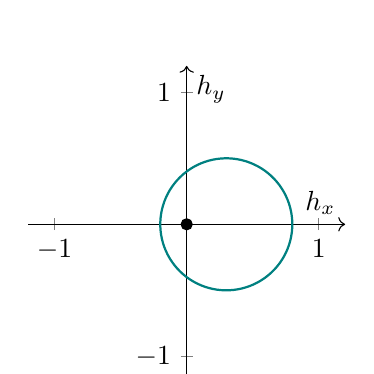
\begin{tikzpicture}
			\begin{axis}[
				axis equal image,
				axis lines=middle,
				axis line style={->},
				xtick={-1,1}, ytick={-1,1},
				xmin=-1.2, xmax=1.2,
				ymin=-1.2, ymax=1.2,
				xlabel=$h_x$, ylabel=$h_y$,
				width=6.5cm,
				]
				\addplot+[mark options={black}] coordinates {(0,0)};
				\addplot [
				samples=100, domain=0:2*pi, color=teal, thick,
				] ( {.5*cos(deg(x)) + 0.3}, {.5*sin(deg(x))} );
			\end{axis}
		\end{tikzpicture}
		\caption{$v=0.3$, $w=0.5$}
	\end{subfigure}
	\caption{Contours in Hamiltonian space for (a) trivial, (b) conducting and (c) topological phases.}
	\label{fig:phases}
\end{figure}

We are now in a position to start analysing the physics of the system. Concretely, the momentum space Hamiltonian is given by
\begin{align*}
	H(k) &= \h(k)\cdot\bm{\upsigma} = \big(v + w\cos(k)\big)\sigma_x + w\sin(k)\sigma_y = \begin{pmatrix}
		0 & v + w\e^{-ik} \\
		v + w\e^{ik} & 0
	\end{pmatrix}.
\end{align*}
We can set up a Fourier transform to real space by rewriting this suggestively in terms of the unit cell index $n$:
\[
	H(k) = \e^{-ik(n-n)}\begin{pmatrix}
		0 & v \\
		v & 0
	\end{pmatrix} + \e^{-ik\big((n+1)-n\big)}\begin{pmatrix}
		0 & w \\
		0 & 0
	\end{pmatrix} + \e^{-ik\big(n-(n+1)\big)}\begin{pmatrix}
		0 & 0 \\
		w & 0
	\end{pmatrix}
\]
{\color{red} I need to work out the details of this Fourier transform later, my calculations aren't working out. Transforming from a periodic Brillouin zone to (discrete or infinite) real space is breaking my brain. I imagine it needs to look something like this (where $M_{0/\pm1}$ are the three matrices above):
\begin{align*}
	\hat{H} &= \int_B H(k) \ket{k}\bra{k} \\
		&= \int_{-\pi}^{\pi}\frac{\dd{k}}{2\pi} \left(\sum_{a\in\{0,\pm1\}}\e^{-ika}M_a\right) \left(\sum_{n}\e^{-ikn}\ket{n}\right) \left(\sum_{n'}\bra{n'}\e^{ikn'}\right) \\
		&= \sum_{a,n,n'}\left(\int_{-\pi}^{\pi}\frac{\dd{k}}{2\pi}\e^{-ik(a+n-n')}\right)M_a\ket{n}\bra{n'} \\
		&= \sum_{a,n,n'}\delta_{n+a,n'}M_a\ket{n}\bra{n'} \\
		&= \sum_{a,n}M_a\ket{n}\bra{n+a}
\end{align*}
But I don't fully understand the first step, the sign of $a$ is wrong and normalization is broken. Maybe it's easier to discretize first and do a DFT?}

{\color{blue}
\begin{itemize}
	\item It follows [how exactly?] that we can write the Hamiltonian in a unit cell basis as
	\[
		\hat{H} = \sum_{n=-\infty}^{\infty}\left[\ket{n}\bra{n}\otimes\begin{pmatrix}
			0 & v \\
			v & 0
		\end{pmatrix} + \left(\ket{n+1}\bra{n}\otimes\begin{pmatrix}
			0 & w \\
			0 & 0
		\end{pmatrix} + {\rm h.c.}\right)\right]
	\]
	
	\item Mention tight binding somewhere around this point
\end{itemize}
}

This Hamiltonian contains a term which acts within the unit cells, and terms which act between neighbouring unit cells, parametrized by $v$ and $w$ respectively. The structure of these interactions can be made somewhat more transparent by going to a finite chain of length $N$. The Hamiltonian then becomes
\[
	\hat{H} = \sum_{n=0}^{N}\ket{n}\bra{n}\otimes\begin{pmatrix}
		0 & v \\
		v & 0
	\end{pmatrix} + \sum_{n=0}^{N-1}\left(\ket{n+1}\bra{n}\otimes\begin{pmatrix}
		0 & w \\
		0 & 0
	\end{pmatrix} + {\rm h.c.}\right),
\]
where open boundary conditions have been introduced on the ends of the chain to allow the boundary behaviour to be studied. The tensor products can be expanded in order to cast the Hamiltonian into a full $2N\times 2N$ matrix:
\[
	\hat{H} = \begin{pNiceMatrix}
		\Block[borders={bottom,right,tikz=dashed}]{2-2}{}
					 0 & v & \Block[borders={bottom,right,tikz=dashed}]{2-2}{}
							 0 & 0 & \Block{4-4}{0} &        &   & \\
					 v & 0 & w & 0 &                &        &   & \\
		\Block[borders={bottom,right,tikz=dashed}]{2-2}{}
					 0 & w & 0 & v &                &        &   & \\
					 0 & 0 & v & 0 &                &        &   & \\
		\Block{4-4}{0} &   &   &   &                & \Ddots & 0 & 0 \\
					   &   &   &   & \Ddots         &        & w & 0 \\
					   &   &   &   &              0 & w      & 0 & v \\
					   &   &   &   &              0 & 0      & v & 0
	\end{pNiceMatrix}.
\]
A physical interpretation of this system presents itself in the form of this matrix: it describes a chain of $2N$ sites, with alternating hopping amplitudes $v$ and $w$ between neighbouring sites. The unit cells now consist of two of these sites, and $v$ and $w$ are referred to as the \emph{intra-cell} and \emph{inter-cell} hoppings, respectively. When these two hoppings are equal, the system is in the gapless phase $v=w$, corresponding to a chain where all bonds are equally strong. Intuitively, this homogeneity allows electrons to propagate freely along the chain. On the other hand, in the insulating cases $v\neq w$, one of the two hoppings is stronger than the other, and the electrons tend to be confined around these stronger bonds.

Dividing the unit cells into two individual sites in this way allows us to distinguish two so-called \emph{sublattices} of the crystal, which we label $A$ and $B$. The notation can then be simplified by labelling quantum states according to the sublattice on which they are localized:
\[
	\ket{n,A} \equiv \ket{n}\otimes\begin{pmatrix}
		1 \\ 0
	\end{pmatrix},\quad \ket{n,B} \equiv \ket{n}\otimes\begin{pmatrix}
		0 \\ 1
	\end{pmatrix}.
\]
In this notation, the Hamiltonian becomes
\begin{equation}\label{eq:ssh-sublattice}
	\hat{H} = \left(\sum_{n=0}^{N}v\ket{n,B}\bra{n,A} + \sum_{n=0}^{N-1}w\ket{n+1,A}\bra{n,B}\right) + {\rm h.c.}
\end{equation}

The tight-binding model of alternating hoppings is precisely the SSH model: it was introduced in 1979 by Wu-Pei Su, John Robert Schrieffer, and Alan J. Heeger to describe polyacetylene (Figure \ref{fig:polyacetylene}), a polymer chain which features alternating single and double covalent bonds \cites{SSH_model}{SSH_model2}.
\begin{figure}[htb!]
	\centering
	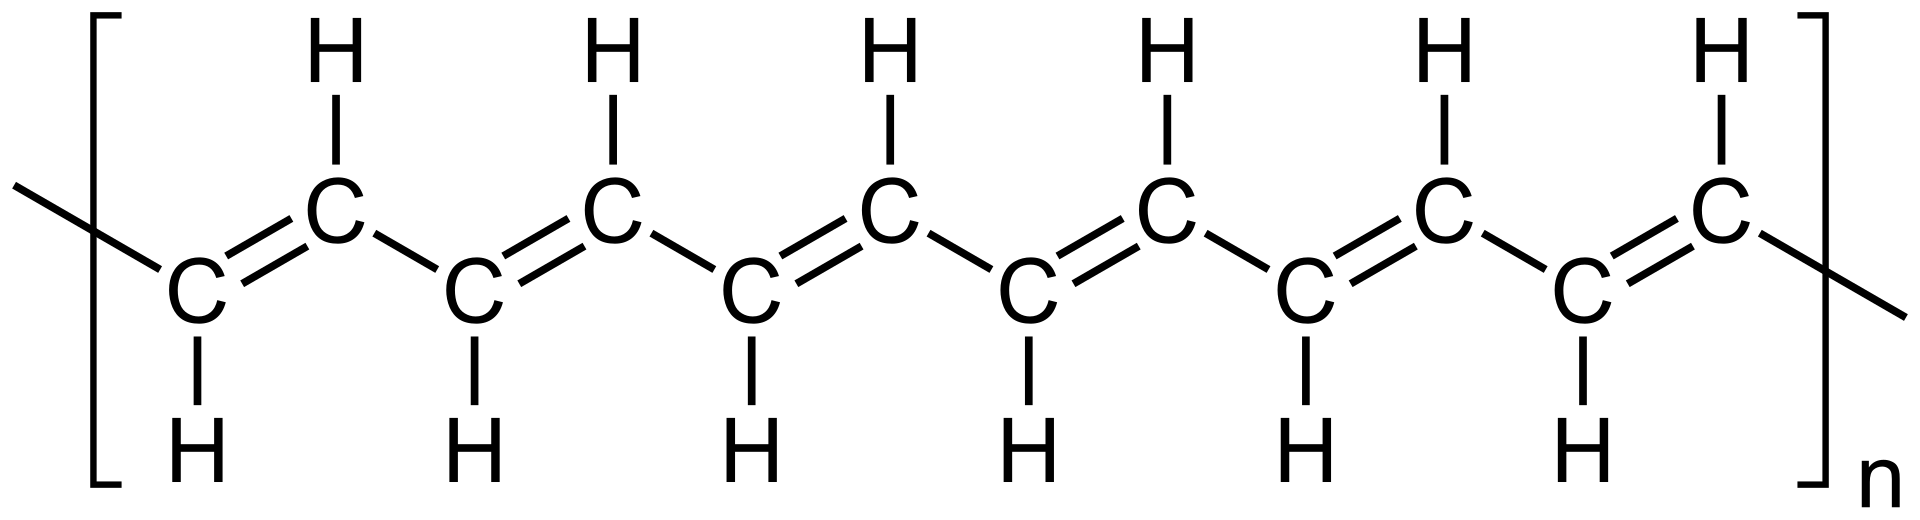
\includegraphics[width=.8\linewidth]{Images/polyacetylene} %TODO svg
	\caption{Structural diagram of polyacetylene. Electrons are transported more readily along the double bonds, which is modelled using a larger hopping parameter.}
	\label{fig:polyacetylene}
\end{figure}
This material displays unexpectedly high conductivity when doped with halogen impurities, and the SSH model affords an explanation for this.

To understand how this metallic behaviour comes about, the differences between the trivial and the topological phase must be examined more closely. The two phases appear to be identical at a first glance: if the unit cell in polyacetylene is chosen in such a way that the stronger double bond represents the intra-cell hopping $v$, then the system is in the trivial phase $v>w$, and if instead the unit cell is centred around a single bond, $v<w$ and the phase is topological. In either case, valence electrons are expected to remain localized around the double bonds, leading to the same insulating bulk behaviour.\footnote{
	The attentive reader might wonder why the conducting $v=w$ phase does not occur naturally in this system. This is a result of the so-called Peierls transition: in a nutshell, introducing a band gap locally lowers the energy of the (filled) valence band and raises that of the (empty) conduction band. This makes it energetically favourable for atoms in the chain to pair up, in a process referred to as dimerisation.}

The difference between the two phases only becomes apparent when the endpoints of the chain are studied. \red{[introduce a figure here]}%TODO
For example, the leftmost atom is not subject to any inter-cell hopping, and it is only connected to the other atom in its unit cell. In the trivial case, this connection is strong and the two atoms share their valence electrons. In the topological phase, on the other hand, the second atom from the left prefers to share electrons with its right-hand neighbour, and the leftmost atom becomes isolated. In the limit where $v$ goes to zero, this isolation becomes complete and the edge sites carry zero-energy eigenstates. In this case, only the second term in the Hamiltonian \eqref{eq:ssh-sublattice} survives, and the edges obey the eigenvalue equations
\begin{align*}
	\hat{H}\ket{1,A} = \hat{H}\ket{N,B} = 0.
\end{align*}
These edge modes can be shown to persist for non-zero $v<w$, in which case they become highly localized and approach zero energy in the $N\to\infty$ limit.\footnote{
	A precise understanding of this is beyond the scope of this review; the interested reader is referred to e.g.\ \cite{Asboth_topo-course}.}
The salient point is that the boundary modes of the topological phase exist inside the energy gap: their energy eigenvalues have a degeneracy at the Fermi level $\varepsilon_F = 0$. \red{[Perhaps include dispersion figure]}
%TODO picture?

Something remarkable has happened: we have started from a topological description of a gapped bulk phase, and the resulting physical effects appear as in-gap zero energy modes on the boundary of the material. As will become apparent looking at other examples, the existence of edge modes at the Fermi level is a fairly\footnote{
	This is not a completely general statement: topological phases with edge modes at energies other than $\varepsilon_F$ have been shown to be theoretically feasible \cite{Freedman_gapped-edge}. For our purposes, it will be sufficient to restrict our attention to edge modes at the Fermi level.}
general feature of topological phases of matter, captured in the so-called \emph{bulk-boundary correspondence}. It can be thought of as being a result of the inability to go continuously from a topological gapped phase to a trivial one in real space; in particular, the outside boundary of an idealised material connects to the vacuum, which is also considered a trivial gapped phase.

{\color{blue}
\begin{itemize}
	\item Discuss physics of polyacetylene (solitons on trivial/topological interface) and experimental observations of solitons + berry phase \cites{Meier_SSH-soliton}{Atala_SSH-Zak}
	
	\item We can now physically interpret the meaning of setting $h_z = 0$: it ensures that hopping only occurs between the two sublattices $A$ and $B$, and not within them (i.e.\ there are only off-diagonal elements in the internal degrees of freedom). If we define the sublattice projection operators
	\[
		\hat{P}_A = \mathbb{I} \otimes \begin{pmatrix}
			1 & 0 \\ 0 & 0
		\end{pmatrix},\quad \hat{P}_B = \mathbb{I} \otimes \begin{pmatrix}
			0 & 0 \\ 0 & 1
		\end{pmatrix}
	\]
	then the Hamiltonian obeys
	\[
		\hat{P}_A\hat{H}\hat{P}_A = \hat{P}_B\hat{H}\hat{P}_B = 0
	\]
	and so since $\hat{P}_A + \hat{P}_B$ is the identity we have
	\begin{align*}
		\hat{H} &= (\hat{P}_A + \hat{P}_B)\hat{H}(\hat{P}_A + \hat{P}_B) \\
			&= \hat{P}_A\hat{H}\hat{P}_B + \hat{P}_B\hat{H}\hat{P}_A \\
			&= (\hat{P}_A - \hat{P}_B)\hat{H}(\hat{P}_B - \hat{P}_A) \\
			&\equiv -\hat{\Gamma}\hat{H}\hat{\Gamma}
	\end{align*}
	with $\hat{\Gamma}\equiv\hat{P}_A - \hat{P}_B$ having the property that $\hat{\Gamma} = \hat{\Gamma}^{-1} = \hat{\Gamma}\dagger$; this is called sublattice symmetry and it also applies to the momentum space Hamiltonian $H(k)$.
	
	\item An immediate consequence of our setup is that the trivial and topological phase become adiabatically connected if we allow for sublattice symmetry breaking ($h_z \neq 0$).
	
	\item Talk more about $\Z$ invariant (next-nearest-neighbour hopping etc.)
\end{itemize}
}

%\subsection{The Kitaev chain}
%
%{\color{blue}
%\begin{itemize}
%	\item Introduce Majorana modes
%	
%	\item Talk about superconductivity
%	
%	\item Discuss $\Z_2$ invariant vs.\ $\Z$ for SSH topologically
%\end{itemize}
%}


\section{Two-dimensional models}

\subsection{Quantum Hall effect}

\subsection{The Chern insulator}\label{sec:Chern}

\subsection{The Kane--Mele model}


\markedsection{Symmetry classes}{Classification of symmetries}
	
\chapter{Weyl semimetals}

\section{Physical aspects}


\section{Topological description}\label{sec:semimetal-topology}

%TODO introductory paragraph

\subsection{3D Chern insulators}

To get a good intuition for the topological description of Weyl semimetals, it is useful to first consider a fully insulating material with similar properties. Suppose we have a three-dimensional material that is not subject to any additional symmetries. Such a material is called a 3D Chern insulator, in analogy to the 2D Chern insulator studied in Section \ref{sec:Chern}.%TODO
This system is not a semimetal in the sense that there are no band crossings in the bulk; still, in many respects it can be considered a limiting case of a Weyl semimetal, where the number of Weyl points is zero. %TODO figure out acceptable wording

From the Atland--Zirnbauer classification in Table \red{[reference]},%TODO
one might expect a 3D Chern insulator to be topologically trivial. However, as seen before in equation \red{[reference] (and perhaps also in 3D BHZ/Kane--Mele if I discuss this in ch. 2)},%TODO
the full topological classification of materials depends not only on the top-dimensional topology, but also on that borrowed from lower-dimensional subspaces. In the case of a 3D Chern insulator, this topology arises on two-dimensional slices of the Brillouin zone; an example of such a slice is highlighted in Figure \ref{fig:3D_Chern_insulator}.
\begin{figure}[htb!]
	\centering
	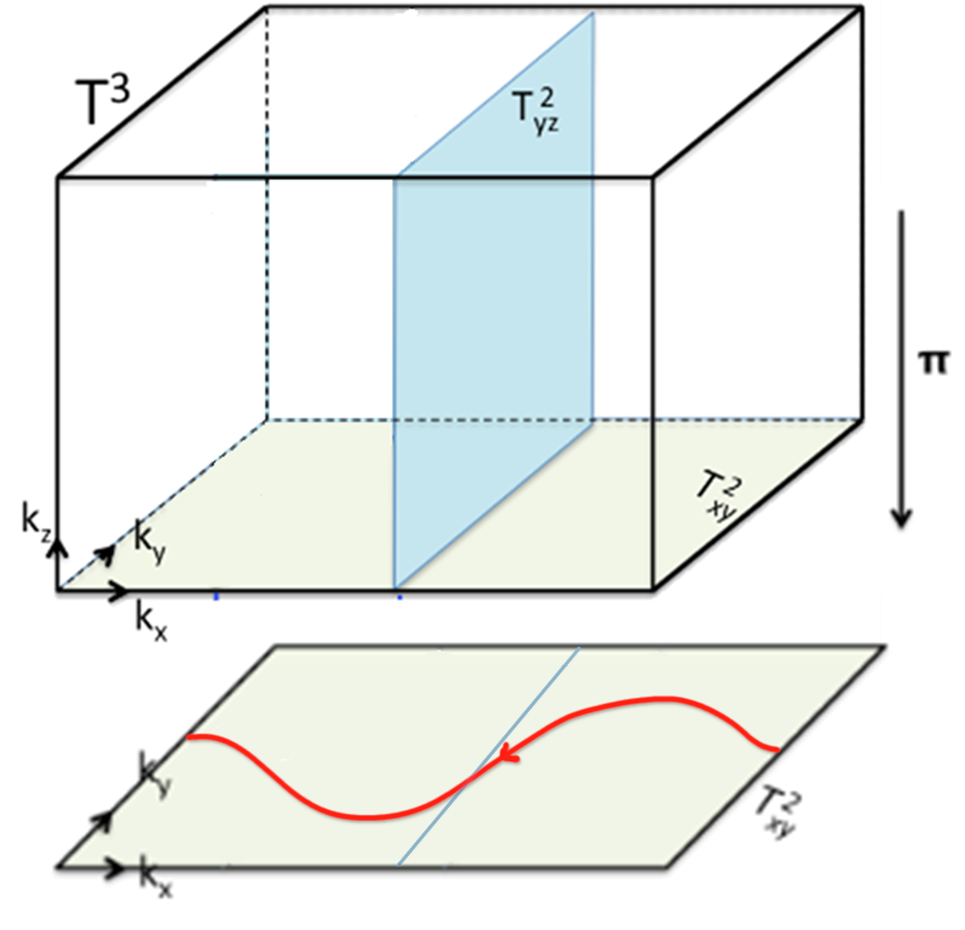
\includegraphics[width=.5\linewidth]{Images/3D_Chern_insulator}
	\caption{
		\red{[Temporary figure]} %TODO fix
		Three-dimensional Brillouin torus $\T^3$ of a Chern insulator, with a two-dimensional slice $\T_{yz}^2$ indicated in blue. A projection onto a surface Brillouin zone in the $xy$-direction is also shown, with an example Fermi loop of gapless states in red. In this example, the slice $\T_{yz}^2$ has a Chern number of $C_{x} = 1$. Hence, its projection onto the surface is a 1D loop that features one band crossing.
		Figure adapted from \cite{Mathai_math-review}.}
	\label{fig:3D_Chern_insulator}
\end{figure}

There are three topologically distinct ways to slice up the three-torus, all perpendicular to one of the three coordinate directions.\footnote{
	Other 2D slices exist, such as those going diagonally across, but these can all be considered linear combinations of the three ``orthogonal'' slices. To be precise, the different classes of 2D subspaces of $\T^3$ form the second homology group $H_2(\T^3)\cong\Z^3$, and this group is \emph{generated} by the orthogonal slices.}
These slices have the topology of a two-torus $\T^2$, and a Chern number can be obtained by integrating the Berry curvature $\Fc$ of the system over them: for example, perpendicular to the $x$ direction there is a Chern number $C_{x} = \int_{\T_{yz}^2}\mathcal{F}$.\footnote{
	Note that it does not matter where along the Brillouin zone this $yz$-slice is taken: the Chern number is an integer, while the system is continuous. This means the $x$ coordinate can be changed continuously without changing the resulting Chern number.}
This results in a classification by three distinct Chern numbers $C_x$, $C_y$ and $C_z$, and in the literature (e.g. \cites{Vanderbilt_2018}{Liu_photonic-Chern-vector}) these are commonly arranged in a so-called \emph{Chern vector}
\[
	\vb{C} = \begin{pmatrix}
		C_x \\ C_y \\ C_z
	\end{pmatrix} \in \Z^3.
\]

Importantly, these three Chern numbers are all induced by a single two-form $\Fc$. In this sense, there is an exact correspondence between topologically distinct Berry curvatures $\Fc$ and Chern vectors $\vb{C}\in\Z^3$. This is precisely what motivates the use of cohomology for classification: just like in the 2D Chern insulator, the two-form $\Fc$ can be considered to represent a class in the second cohomology group,
\begin{equation}\label{eq:2nd-cohom-t3}
	[\Fc]\in H^2(\T^3)\cong\Z^3. 
\end{equation}
As a result, this group precisely classifies the distinct topological phases of the system.\footnote{
	More fundamentally, a complex vector bundle called the \emph{valence bundle} can be associated to a gapped Hamiltonian, and the second cohomology group classifies the different complex vector bundles over a manifold.}

\subsubsection{Boundary states}

Before moving on to a system with Weyl points, it will be instructive to study the gapless modes that arise on the surface of a 3D Chern insulator with non-zero Chern vector. Figure \ref{fig:3D_Chern_insulator} illustrates the case where $\vb{C} = (1,0,0)\tran$. In this case, $\T_{yz}^2$ is the only orthogonal slice with a non-zero Chern number, and as such the material lattice can be thought of as a stack of 2D Chern insulators spanning the $y$ and $z$ directions, stacked together in the $x$ direction. $\T_{yz}^2$ can effectively be considered the Brillouin zone of such a 2D Chern insulator.

Recall from our discussion in Section \ref{sec:Chern} that a 2D Chern insulator with a Chern number of 1 has a single chiral edge mode, which manifests as a gapless state on the one-dimensional surface Brillouin zone. %TODO Extra canceling edge modes may appear <=> folding of the Fermi loop
This logic can be translated to the the three-dimensional case, where such slices are stacked in the $x$ direction. Suppose there is a projection $\pi$ along the $z$ direction, onto a two-dimensional surface Brillouin zone $\ext{\T}_{xy}^2$. Then the two-dimensional slices $\T_{yz}^2$ project down to a one-dimensional loop $\pi(\T_{yz}^2)\cong S^1$ containing a single point-like gapless state. As the $\T_{yz}^2$ slice is moved around in the $x$ direction, this band crossing point moves continuously along the $y$ direction, by continuity of the Hamiltonian. It follows that the full two-dimensional surface Brillouin zone must contain a loop of gapless states going across the $x$ direction, as depicted in the figure. This loop is called a Fermi loop, in analogy with the Fermi arcs in a Weyl semimetal, and the existence of such loops is experimentally well documented \red{[references]}. %TODO refs
Moreover, the chirality of the edge modes can be used to assign a consistent orientation to this loop. %TODO note about linked loops, extra topology etc.

Fermi loops admit a natural topological description in terms of homology. Being oriented loops, they precisely represent a class in the first homology group $H_1(\ext{\T}^2)$ of the surface Brillouin zone. Furthermore, it is possible to define an oriented \emph{Dirac loop} \red{[I don't know if there is an established term for this]} %TODO terminology
$\ell$ in the bulk Brillouin zone in such a way that its projection $\pi(\ell)$ onto the surface in any direction is exactly the Fermi loop. This loop $\ell$ is not a gapless feature \red{[it does seem to be related to gauge singularities, at least in WSMs]}, %TODO
but it is rather interesting topologically: it represents a first homology class in the bulk Brillouin zone,
\[
	[\ell]\in H_1(\T^3)\cong\Z^3.
\]

It is not a coincidence that this first homology group is isomorphic to the second cohomology group $H^2(\T^3)$ from Equation \eqref{eq:2nd-cohom-t3}. This equivalence is a result of \emph{Poincar\'e duality}, which is the statement that for any closed oriented $d$-dimensional manifold $M$, the isomorphism
\[
	H_n(M) \cong H^{d-n}(M)
\]
holds for any integer $n$. In the present case, this duality can be stated intuitively in terms of Chern numbers, which count the number of signed intersections of the Dirac loop with the different two-dimensional slices of the Brillouin zone. This duality can be summarised schematically as follows:
\begin{equation}\label{eq:duality-scheme}
	H^2(\T^3) \ni [\Fc] \overset{\rm integration}{\iff} %TODO change "integration"?
	\vb{C} \overset{\rm intersections}{\iff} [\ell] \in H_1(\T^3).
\end{equation}
This Poincar\'e duality ensures that the classifications in terms of first homology and second cohomology are completely equivalent in this case. Importantly, however, Poincar\'e duality depends on orientability, and it will not hold when we consider non-orientable Brillouin zones in the next chapter. As such, the question of which group provides the right classification of such a system will be key. For the moment, we turn our attention to the topology of Weyl points in the simpler orientable setting.


\subsection{Introducing Weyl points}

Consider a Weyl semimetal with a set of $k$ Weyl points
\[
	W \equiv \set{w_1,w_2,\ldots,w_k}\subset \T^3.
\]
Then the charge of a Weyl point $w_i$ is given by the Chern number
\begin{equation}
	C_w = \int_{S_w^2}\!\Fc,
\end{equation}
where $S_w^2$ is a sufficiently small 2-sphere centred at $w$---in particular, it must be small enough to contain no other Weyl points in its interior. Naively, this might lead us to expect that a semimetal phase is classified by the second cohomology group of the collection of all these spheres:
\begin{equation}\label{eq:2nd-cohom-spheres}
	H^2\left(\bigcup_{i=1}^k S_{w_i}^2\right)\cong \bigoplus_{i=1}^k H^2(S_{w_i}^2) \cong \Z^k.
\end{equation}
However, this classification runs into two problems: it ignores the global cancellation of charge, and it also ignores the additional topology on two-dimensional slices discussed in the previous subsection. Both of these issues are due to the fact that this group only captures the \emph{local} topology near each Weyl point, and they can be addressed by studying how the different Chern numbers on the Brillouin zone must relate to each other \emph{globally}.

The Nielsen--Ninomiya charge cancellation theorem is one such global relation. It is the statement that all the Chern numbers on these 2-spheres must add to zero:
\begin{equation}
	\sum_{i=1}^{k}C_{w_i} = 0.
\end{equation}
This cancellation can be demonstrated using Stokes' theorem. The argument goes as follows: imagine that the interior of each sphere $S_{w_i}^2$ (i.e.\ a small open 3-ball centred at $w_i$) is removed from $\T^3$. The resulting 3-manifold $X$ looks like a 3-torus with $k$ small ball-shaped holes, and its boundary is given by the collection of spheres:
\[
	\partial X = -\bigcup_{i=1}^k S_{w_i}^2,
\]
where the minus sign induces the correct orientation. Then Stokes' theorem gives
\[
	0 = \int_{\partial X} \dd{\Fc} = -\sum_{i=1}^{k}\int_{S_{w_i}^2}\!\!\Fc = -\sum_{i=1}^{k}C_{w_i},
\]
which is precisely the Nielsen--Ninomiya theorem.

A similar argument can also be applied to study what happens to Chern numbers on two-dimensional slices of the Brillouin zone in this context. This argument is illustrated in Figure \ref{fig:Weyl-point-Stokes}.
\begin{figure}[htb!]
	\centering
	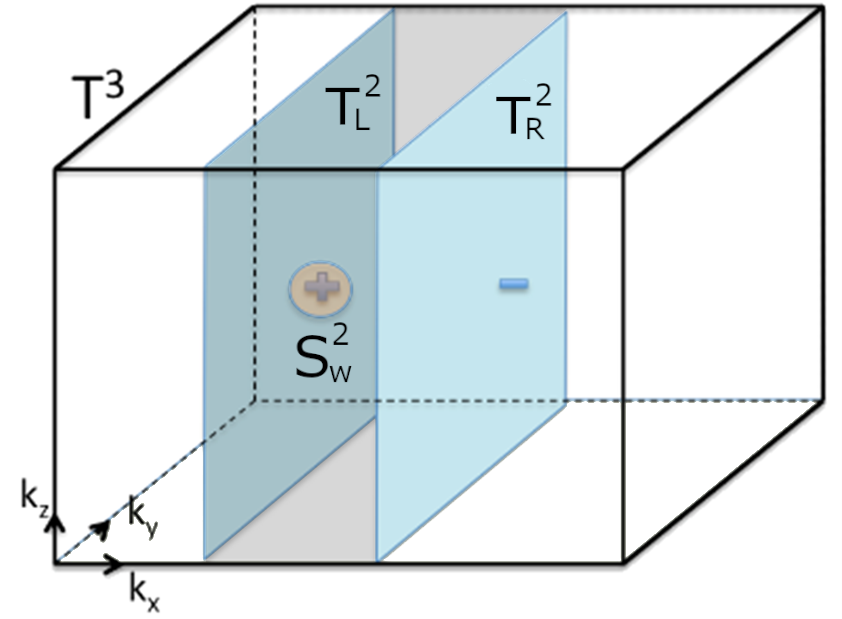
\includegraphics[width=.5\linewidth]{Images/Weyl-point-Stokes}
	\caption{
		Brillouin torus $\T^3$ of a Weyl semimetal with two oppositely charged Weyl points labelled $+$ and $-$. Three two-dimensional subspaces are indicated in blue: a $yz$-like 2-torus on either side of the $+$ point, and a small 2-sphere surrounding it. Given the proper orientation, the blue spaces form the boundary of a three-dimensional manifold $Y$, shaded in grey here.
		Figure from \cite{Mathai_math-review}. \red{[not yet licensed; may need better labelling]}%TODO
	}
	\label{fig:Weyl-point-Stokes}
\end{figure}
Here two slices $\T_L^2$ and $\T_R^2$ are placed on either side of a Weyl point $w$ with charge $C_w = q$, along with a small sphere $S_w^2$ surrounding it. These spaces then bound a three-dimensional manifold $Y$ as indicated in the figure, given the following orientations:
\[
	\partial Y = \T_R^2 - \T_L^2 - S_w^2.
\]
The same Stokes' theorem argument can then be used to relate the Chern numbers $C_L$ and $C_R$ on the respective slices, yielding
\[
	C_R = C_L + C_w = C_L + q.
\]
That is, the Chern number of a two-dimensional slice increases by $q$ every time it passes over a Weyl point with charge $q$. As a sanity check, it should be noted that this process respects the periodicity of the Brillouin torus: when the slice is passed over the entire torus, charge cancellation ensures that the added Chern number is zero in total.

All in all, the presence of Weyl points allows for a finer collection of Chern numbers to appear in the Brillouin zone, beyond the $\Z^3$ Chern vector of the insulating case. This behaviour can be captured using cohomology. The key idea is that the Berry curvature has a singularity at points where the gap closes.\footnote{
	Note that this singularity is required in order for the Chern number to change suddenly when a slice (i.e.\ the integration domain of $\Fc$) is moved over a Weyl point continuously.}
As such, it can only be integrated over subspaces where the gap never closes, so that the set of Weyl points $W$ needs to be excluded. This means $\Fc$ now lives in the second cohomology group of the Brillouin zone minus $W$:
\begin{equation}\label{eq:2nd-cohom-semimetal}
	[\Fc]\in H^2\big(\T^3\setminus W\big) \cong \Z^3\oplus\Z^{k-1},
\end{equation}
where $k$ again is the number of Weyl points. Put differently, classification of semimetallic phases given a set of Weyl points $W$ essentially amounts to classifying the gapped phases on the punctured torus $\T^3\setminus W$.

Notably, this classification addresses both issues present in the $\Z^k$ classification on 2-spheres in Equation \eqref{eq:2nd-cohom-spheres}. Firstly, it incorporates 3D Chern insulator topology in the first term, in the form of the $\Z^3$ from Equation \eqref{eq:2nd-cohom-t3}. Perhaps more subtly, charge cancellation is also incorporated in the form of the reduction by one $\Z$ factor in the second term. This can be understood intuitively: for example, if $k=1$ then the Nielsen--Ninomiya theorem implies that the single Weyl point must have a charge of 0, and so it is not topologically protected. A similar intuition holds for larger $k$, in that the $k$ additional ``degrees of freedom'' which are afforded to the system by the Weyl point charges are reduced by one under the charge cancellation condition. This relation will become more explicit once the Mayer--Vietoris sequence is introduced in Section \ref{sec:Mayer-Vietoris}.

%Notably, there are $k-1$ extra factors of $\Z$ involved in the classification of a Weyl semimetal compared to that of a 3D Chern insulator (cf.\ Equation \eqref{eq:2nd-cohom-t3}). This contrasts with the $k$ factors found for the collection of spheres in Equation \eqref{eqeq:2nd-cohom-spheres}. This reduction by one is a natural result of charge cancellation: for example, if $k=1$ then the Nielsen--Ninomiya theorem implies that the single Weyl point must have a charge of 0, and so it is not topologically protected. A similar intuition holds for general $k\in\N$, in that the $k$ additional ``degrees of freedom'' which are afforded to the system by the Weyl point charges are reduced by one under the charge cancellation condition. This relation will become more explicit once the Mayer--Vietoris sequence is introduced in Section \ref{sec:Mayer-Vietoris}.


\subsubsection{Fermi arcs}

The varying Chern numbers over Weyl points help explain how Fermi arcs arise on the surface. As discussed in the case of a 3D Chern insulator, Fermi loops on the surface arise whenever there is a non-zero Chern number in some direction. Similarly, Fermi arcs begin and terminate whenever the presence of a Weyl point causes a change in the Chern number; this is illustrated in Figure \ref{fig:Fermi-arc-Chern}.
\begin{figure}[htb!]
	\centering
	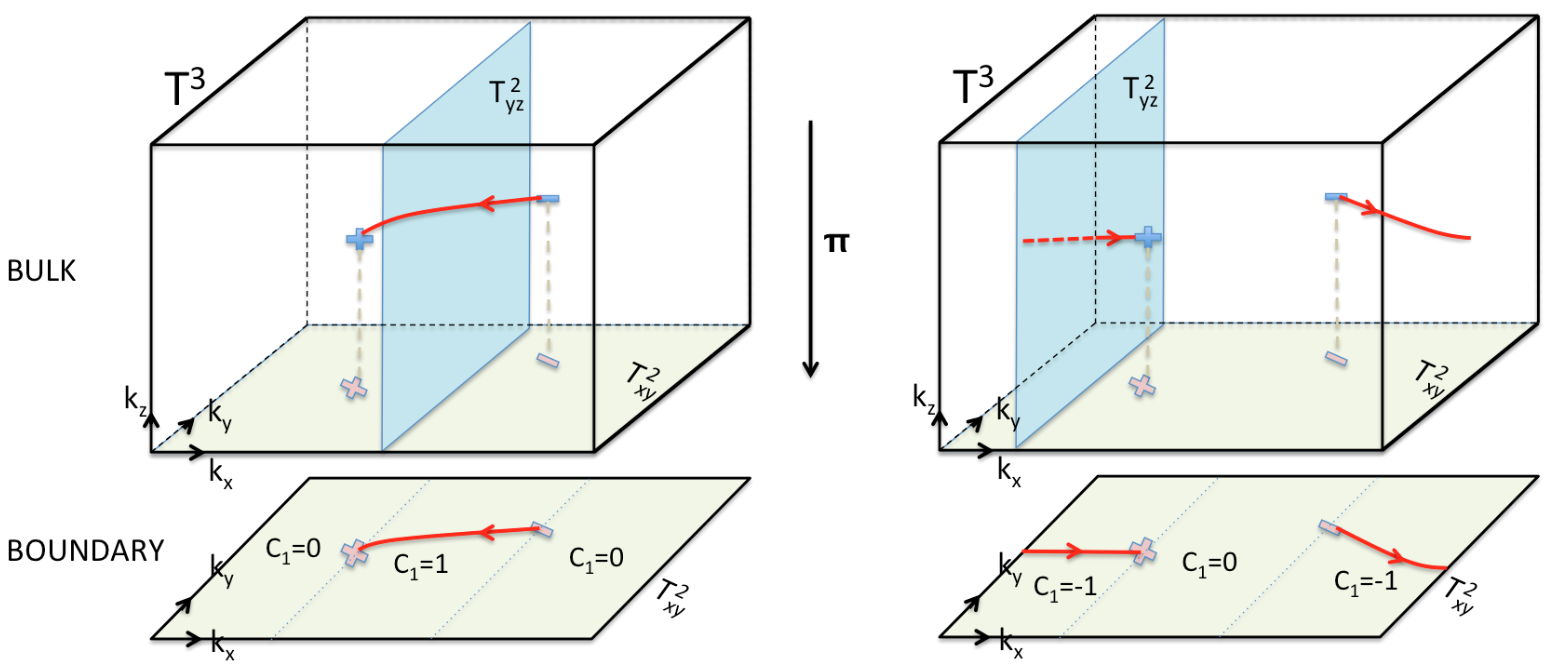
\includegraphics[width=\linewidth]{Images/Fermi-arc-Chern}
	\caption{
		Two semimetal Brillouin zones are shown with the same configuration of Weyl points, but featuring topologically distinct Fermi arcs (shown in red on the boundary). The distinction is due to different bulk Chern numbers: Fermi arcs appear in regions where the bulk Chern number is non-zero. These Fermi arcs can be considered to be the projection of a Dirac string (shown in red in the bulk).
		Figure from \cite{Mathai_math-review}.}
	\label{fig:Fermi-arc-Chern}
\end{figure}

This feature of Weyl semimetals implies they can mediate phase transitions between 3D Chern insulators with different Chern vectors. For example, suppose a pair of Weyl points is created at some point in the Brillouin zone of a trivial insulator ($\vb{C}=0$). These points can then be moved apart in the $z$ direction until they meet again and annihilate at the other end of the torus. In the process, a Fermi arc extends between the projections of the Weyl points on the $xz$ and $yz$-planes, which eventually closes into a Fermi loop. In its final state, the system features a non-zero Chern vector of $\vb{C} = (0,0,1)\tran$. This process was first observed experimentally by Gui-Geng Liu et al.\ in 2022 (see Figure \ref{fig:Weyl-phase-transition}), in the context of a photonic crystal. This was also the first experimental realisation of a 3D Chern insulator \cite{Liu_photonic-Chern-vector}.
\begin{figure}[htb!]
	\centering
	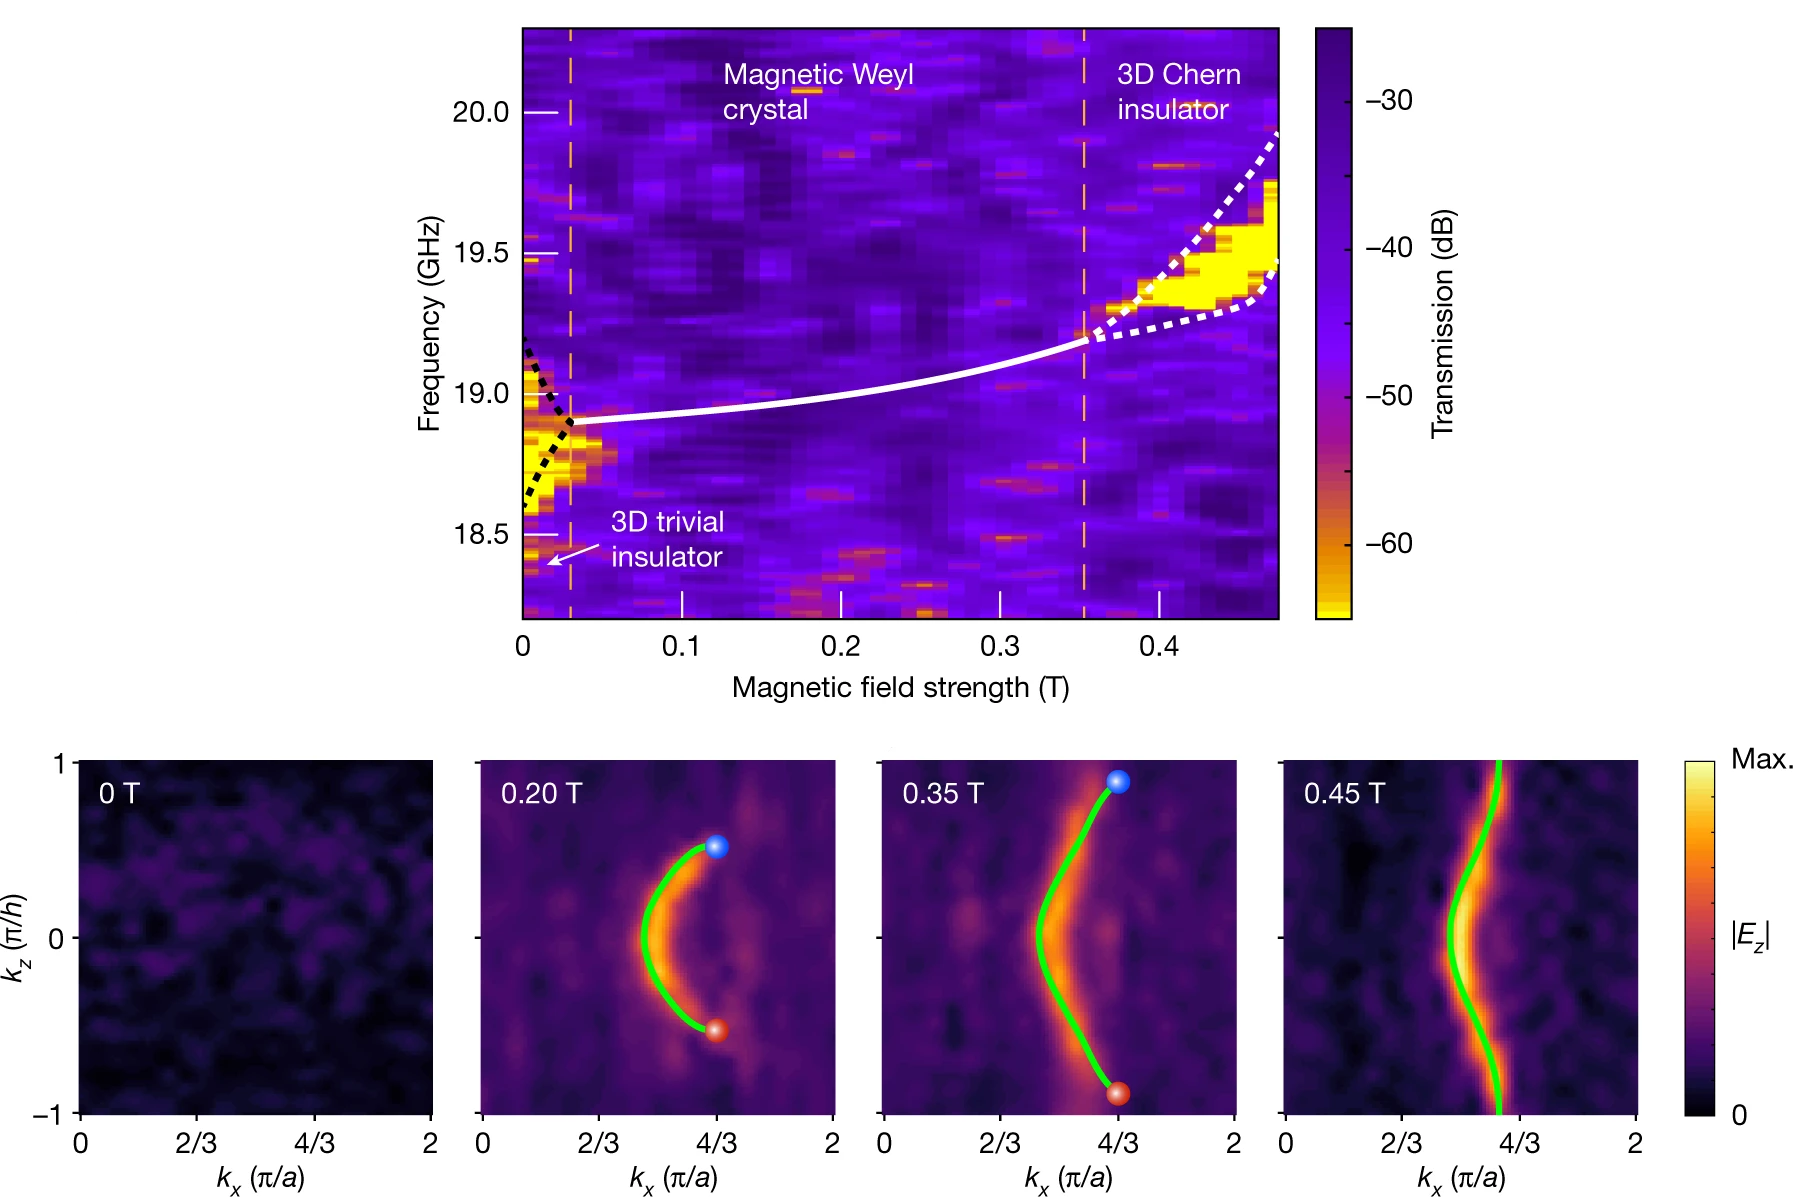
\includegraphics[width=\linewidth]{Images/Weyl-phase-transition}
	\caption{
		\red{[I need to think about how to organise this figure and add a caption]} %TODO
		Figure from \cite{Liu_photonic-Chern-vector}, reproduced with permission from Springer Nature.}
	\label{fig:Weyl-phase-transition}
\end{figure}

Just as Fermi loops can be considered projections of a bulk Dirac loop, so too can Fermi arcs be considered a projection of a bulk \emph{Dirac string}.\footnote{
	A more or less equivalent concept is referred to as \emph{Euler chain} in \cite{Mathai_math-review}, placing the emphasis on topology over physics: ``chain'' here refers the oriented subspaces that homology is founded on.}
Like Dirac loops, these strings can be given an interpretation in terms of homology. The setup is somewhat more subtle in this case: since the Dirac strings have a boundary, they are not loops and as such do not represent homology classes in $H_1(\T^3)$. Instead, they represent classes in the \emph{relative homology group}
\begin{equation}
	H_1\big(\T^3, W\big) \cong \Z^3\oplus\Z^{k-1}
\end{equation}
with respect to the set of Weyl points $W\subset\T^3$. Intuitively, taking the relative homology means that any boundaries lying in the subset $W$ are ignored; for a more precise definition the reader is referred to \parencite[\S 2.1]{Hatcher_algebraic-topology}.

This homology picture provides a classification scheme that is exactly dual to the cohomology classification in Equation \eqref{eq:2nd-cohom-semimetal}; that is, there is an isomorphism
\begin{equation}\label{eq:semimetal-duality}
	H^2\big(\T^3\setminus W\big) \cong H_1\big(\T^3, W\big).
\end{equation}
This is not a direct Poincar\'e duality, but it is nevertheless mathematically rigorous and protected by orientability in the same way.\footnote{
	To be precise, Poincar\'e duality does not hold directly because $\T^3\setminus W$ is not a closed manifold. Instead, for non-compact manifolds $M$ there is a generalized duality $H^n(M)\cong H_{d-n}^{\rm BM}(M)$ where the group on the right is the \emph{Borel--Moore homology}, and this is in turn equivalent to the relative homology in this case. Alternatively, Equation \eqref{eq:semimetal-duality} can be interpreted as a result of the so-called \emph{Lefschetz duality} $H^n(M)\cong H_{d-n}(M, \partial M)$ for manifolds with a boundary.}
The interpretation in terms of Chern numbers given in Equation \eqref{eq:duality-scheme} also still holds here, with the Chern vector and Dirac loops replaced with more general Chern numbers and Dirac strings, respectively.


\subsection{The semimetal Mayer--Vietoris sequence}\label{sec:Mayer-Vietoris}

In the previous section a heuristic Stokes' theorem argument was discussed for charge cancellation on Weyl points. This argument can be generalized by moving to a more abstract cohomology setting, where we are not dependent on the integration of forms; this is important because integration will not be well defined once we move to a non-orientable setting. As an added bonus, the abstract description proves to be richer and provide more detailed information on the possible topological phases for a Weyl semimetal.

The idea is that the relation between the global semimetal topology in Equation \eqref{eq:2nd-cohom-semimetal} and the local charge data in Equation \eqref{eq:2nd-cohom-spheres} can be understood by considering how cohomology classes are mapped between them. That is, one needs to find and study a homomorphism
\begin{equation*}
	\beta: H^2\big(\T^3\setminus W\big) \to H^2\left(\bigcup_{i=1}^k S_{w_i}^2\right).
\end{equation*}
Such a map arises naturally in the context of the \emph{Mayer--Vietoris sequence} for cohomology.

Mayer--Vietoris sequences are used to study how the homology or cohomology of a topological space relates to that of its subspaces. To be precise, let $X$ be a topological space and let $A,B\subset X$ be two subspaces that cover it (i.e.\ $A\cup B = X$). Then there is an \emph{exact sequence} of homomorphisms between cohomology groups,
\begin{equation*}
	\cdots \to H^n(X) \to H^n(A)\oplus H^n(B) \to H^n(A\cup B) \to H^{n+1}(X) \to \cdots,
\end{equation*}
which continues indefinitely in both directions. Exactness means that the image of each map in the sequence is exactly equal to the kernel of the next. In other words, the elements in each term in the sequence which are mapped to zero in the next term are precisely those which ``descend'' from the previous term. In particular, the composition of two subsequent maps always yields zero.

In the context of a Weyl semimetal there is a natural way to divide the Brillouin torus $\T^3$ into two subspaces; this is illustrated in Figure \ref{fig:semimetal-MV}.
\begin{figure}[htb!]
	\centering
	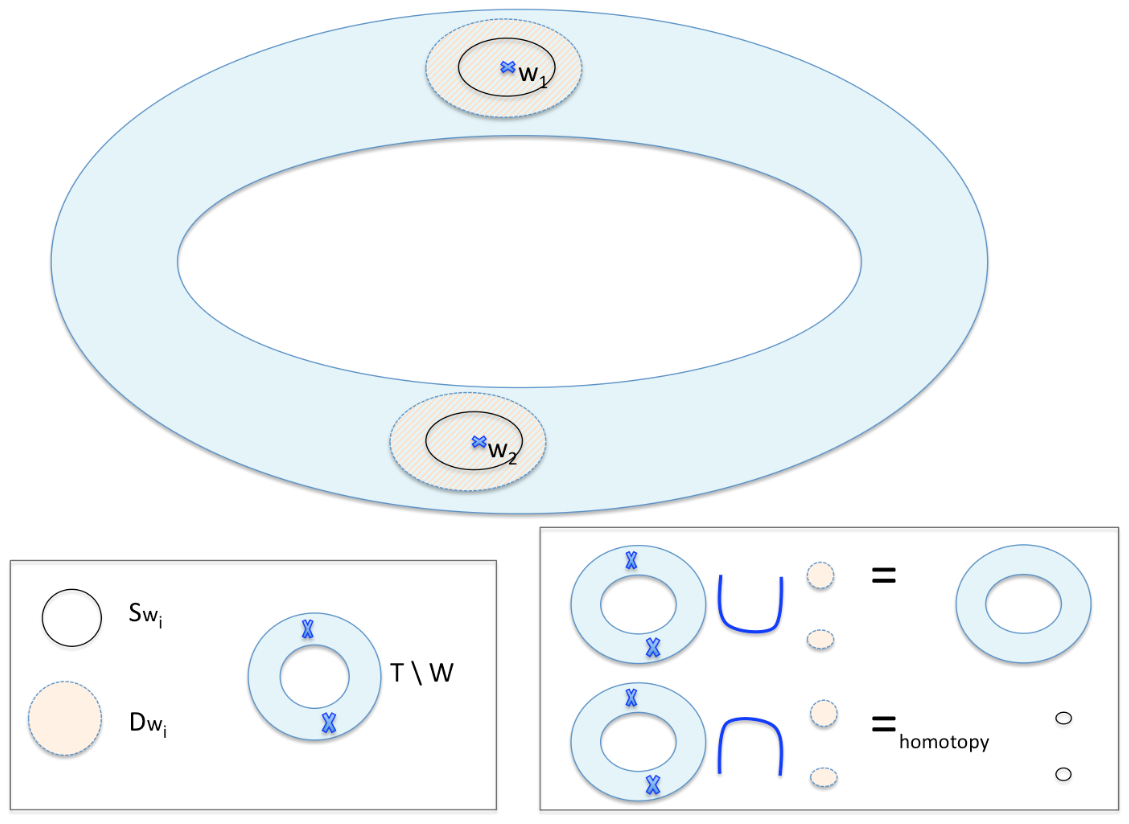
\includegraphics[width=.8\linewidth]{Images/semimetal-MV}
	\caption{
		Schematic two-dimensional representation of the Brillouin torus and the subspaces used to cover it.
		Figure from \cite{Thiang_equivariant}}
	\label{fig:semimetal-MV}
\end{figure}
The first subspace in the covering is the punctured torus $\T^3\setminus W$; we have already encountered this space in classifying topological semimetal phases. The other is the collection $\bigcup_{i=1}^k D_{w_i}^3$ of small open 3-balls centred on the Weyl points $w_i$. The intersection of these two spaces is the same collection of open balls, but each with a single puncture. For our purposes, this intersection has the same topology as the collection of 2-spheres $\bigcup_{i=1}^k S_{w_i}^2$ that we encountered in the context of local Weyl point charges.\footnote{
	To be precise, the punctured 3-balls can be \emph{deformation retracted} into the 2-spheres, making them \emph{homotopy equivalent}. Homotopy equivalent spaces have the same homology and cohomology groups.}
A Mayer--Vietoris sequence can now be written down for these subspaces. The section of this sequence which is relevant to classification is referred to as the \emph{semimetal Mayer--Vietoris sequence}:\footnote{
	Note that the open balls $D_{w_i}^3$ do not appear in this sequence at all. This is because they can be contracted to a point, and hence are topologically trivial in a sense.}
\begin{equation}\label{eq:semimetal-MV-symbolic}
	0\ \to\ \underbrace{H^2(\T^3)}_{\mathclap{\text{3D Chern insulator}}}\ \to\ 
	\underbrace{H^2\big(\T^3\setminus W\big)}_{\text{Semimetal}}\ \overset{\beta}{\to}\ \underbrace{H^2\left(\bigcup_{i=1}^k S_{w_i}^2\right)}_{\text{Local charges}}\ \overset{\Sigma}{\to}\ H^3(\T^3)\ \to\ 0.
\end{equation}
The first three groups in this sequence are already familiar from Equations \eqref{eq:2nd-cohom-t3}, \eqref{eq:2nd-cohom-semimetal} and \eqref{eq:2nd-cohom-spheres} respectively. The last group $H^3(\T^3)\cong\Z$ is represented by volume forms\footnote{
	I.e.\ 3-forms, which are locally proportional to $\dd{k_x}\wedge\dd{k_y}\wedge\dd{k_z}$.}
on the torus; one notable example of such a form is the trivial 3-form
\begin{equation*}
	\dd{\Fc} = 0 \in H^3(\T^3)
\end{equation*}
which appeared in the Stokes' theorem arguments previously. Indeed, the map labelled $\Sigma$ above can be loosely interpreted as the exterior derivative $\dd$. However, a more physically useful interpretation is that $\Sigma$ gives the total charge in the system: it sends a set of Chern numbers on the Weyl points to their sum in $\Z$.

Explicitly, the semimetal Mayer--Vietoris sequence is
\begin{equation}\label{eq:semimetal-MV-explicit}
	0 \to \Z^3 \to \Z^3\oplus\Z^{k-1} \overset{\beta}{\to} \Z^k \overset{\Sigma}{\to} \Z \to 0.
\end{equation}
The exactness of this sequence can be used to extract useful information, especially around the group of local charges $\Z^k$. Here exactness means that $\im(\beta) = \ker(\Sigma)$. This implies that the local charges on the Weyl points sum to zero if and only if they descend from a semimetal. In other words, it implies not only the Nielsen--Ninomiya charge cancellation theorem, but also its converse: any set of Weyl points with charges adding to zero is admissible as a topological Weyl semimetal phase.

In fact, more can be inferred by looking at the maps around the semimetal group $\Z^3\oplus\Z^{k-1}$. Here exactness tells us that $\ker(\beta)\cong\Z^3$. This makes physical sense: if all local charges are zero, the Weyl points are not topologically protected and the system is really in a 3D Chern insulator phase. However, since $\beta$ is a homomorphism, we also find $\beta^{-1}(c)\cong\Z^3$ for a generic charge configuration $c\neq 0\in\Z^k$; that is, every configuration with total charge zero admits a $\Z^3$ worth of topologically different semimetal phases. This makes precise a principle that is also hinted at in Figure \ref{fig:Fermi-arc-Chern}: Weyl semimetals with identical charge configurations may nevertheless be topologically distinct, and their topologies differ by a bulk Chern vector in $\Z^3$.\footnote{
	Properly speaking, the set of topological phases for a given charge configuration is an affine space for $H^2(\T^3)$, since there is no canonical zero Chern vector on a Weyl semimetal. This is worked out in greater mathematical detail in Section 3 of \cite{Mathai_math-review}.}


\subsubsection{The dual homology sequence}

\markedchapter{Non-orientable mfds}{Non-orientable systems}

Symmetries play a crucial role in establishing and differentiating topological properties of physical systems; this much is already evident from the tenfold way classification discussed in Section \ref{sec:symm-classes}. However, in recent years researchers have begun to recognise that symmetries beyond the standard time reversal, charge conjugation and chiral symmetries can give rise to distinct topological invariants that are not fully captured by this classification.

An important class of these extended symmetries is comprised by the space groups acting on periodic lattices. These impose additional structure on the unit cell of the lattice, such as rotational or reflection symmetry. Of special interest here are the so-called non-symmorphic space group symmetries, which combine basic rotation, reflection or inversion with a lattice translation. These symmetries have no fixed points and may induce novel topological states when applied to a material lattice.

Very recently, the feasibility of applying these non-symmorphic symmetries in momentum space has been demonstrated both theoretically and experimentally. This opens up new and interesting avenues of research relating to Brillouin zone topology. In particular, the Brillouin zone may become effectively non-orientable, challenging the notion of chirality for Weyl points.

We begin this chapter with a short review of existing literature surrounding these concepts, culminating in a treatment of a recent paper which applies them to Weyl semimetals. We then present a novel topological analysis of the system described in this paper, in terms of the cohomology and homology tools presented in Chapter \ref{chap:WSM}.

\markedsection{Review}{Review of recent literature}

{\color{blue}
\begin{itemize}
	\item Chen, Yang and Zhao describe a 2D system in Ref.\ \cite{CYZ_Klein-gauge} where the Brillouin zone has the topology of a Klein bottle, induced by the glide symmetry
	\begin{equation}\label{eq:2D_glide}
		UH(k_x, k_y)U\herm = H(-k_x, k_y + \pi)
	\end{equation}
	This system features a $\Z_2$ invariant, as opposed to a $\Z$ Chern number, relating to the fact that $H^2(K^2) = \Z_2$.
	
	\item Other works have verified this experimentally and generalised the theory to higher dimensions and other non-symmorphic symmetries.
\end{itemize}
}

\subsection{Non-orientable Weyl semimetals}

{\color{blue}
\begin{itemize}
	\item Fonseca, Vaidya et al.\ report on the properties of Weyl points in a $K^2\times S^1$ Brillouin zone \cite{Fonseca-Vaidya_nonorientable}. This is achieved using a momentum-space glide symmetry:
	\begin{equation}\label{eq:3D_glide}
		H(k_x, k_y, k_z) = H(-k_x, k_y + \pi, k_z).
	\end{equation}
	An $\R P^2\times S^1$ topology from a double glide symmetry is also discussed in the supplemental material.
	
	\item The fundamental Brillouin zone is parametrised with $k_x,k_z\in[-\pi,\pi]$ and $k_y\in[-\pi,0]$, with the necessary boundary identifications.
	
	\item Emphasis is placed on the "orientation-reversing planes" at $k_y = -\pi$ and $k_y = 0$: moving a Weyl point across one of these planes makes it return on the other side with opposite charge. As a result, there is no absolute notion of chirality on the Klein bottle.
	
	\item The authors still apply a notion of relative chirality, tied to the choice of fundamental domain. With respect to this notion, it is shown that Nielsen--Ninomiya is circumvented: The total chirality of the Weyl points in the fundamental domain may be non-zero.
	
	\item An argument is made relating the breaking of Nielsen--Ninomiya to a claimed discontinuity of the Bloch vector field defining the Hamiltonian.
	
	\item Weyl points with unit charge must still be connected via Fermi arcs; a pair of points with the same charge may be connected by a Fermi arc which crosses the orientation-reversing boundary an odd number of times.
	
	\item A $\Z_2$ invariant is shown to exist on $K^2$-like slices of the EBZ, and it is claimed that this invariant is sourced by the Weyl points.
	
	\item An experimental realisation of the system is demonstrated using 1D photonic crystals with two synthetic momenta.
\end{itemize}
}


\markedsection{Topology}{Topological exploration}\label{sec:non-ori_topology}

%TODO implement feedback

The purpose of this section is to reframe and analyse the non-orientable Weyl semimetals described in Ref.\ \cite{Fonseca-Vaidya_nonorientable} in terms of the algebraic topology language from Chapter \ref{chap:WSM}	. This approach has the advantage of being coordinate-free, and as such it provides a more fundamental understanding of the system's topological properties. We obtain a direct description of how the Nielsen--Ninomiya theorem is modified into a $\Z_2$ charge cancellation condition. We also obtain a more complete picture of the different invariants associated with such a system, and are able to distinguish which are related to the topological insulator phase, and which relate to the introduction of Weyl nodes. To the knowledge of the author, the insights contained in this section are novel.

\subsection{Preliminary clarifications}

As a motivation for the proposed coordinate-free description, we begin by clearing up some minor points of confusion present in Ref.\ \cite{Fonseca-Vaidya_nonorientable}.

First of all, there is a relatively strong emphasis on the two ``orientation-reversing planes'' at $k_y=\pm\pi$ and $k_y=0$. For example, it is stated that relative chirality can be defined unambiguously on fundamental domains that avoid these planes. This is true on a technical level, but it creates the impression that the orientation reversal occurs locally at the boundary of the fundamental domain, raising questions about the nature of Weyl points existing on these planes.

In reality, orientation reversal is a global feature. We are free to reparametrise the fundamental domain in a way that includes the planes $k_y=\pm\pi$ and $k_y=0$, and the notion of relative chirality may change as a result; this is illustrated in Figure~\ref{fig:BZ_param}.
\begin{figure}[htb!]
	\centering
	\subcaptionbox{$-\pi \leq k_y \leq 0$\label{subfig:BZ_basic}} {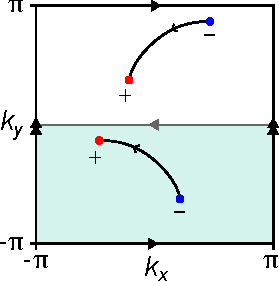
\includegraphics[width=.3\textwidth]{Images/BZ_basic}}
	\hfil
	\subcaptionbox{$-\pi/2 \leq k_y \leq \pi/2$}{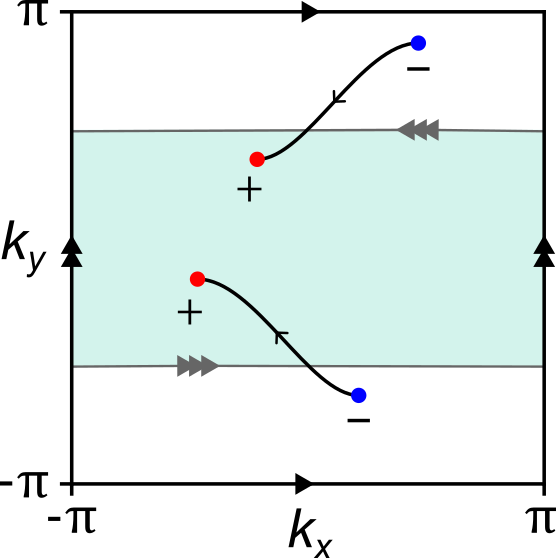
\includegraphics[width=.3\textwidth]{Images/BZ_mid}}
	\hfil
	\subcaptionbox{$-\pi \leq k_x \leq 0$}{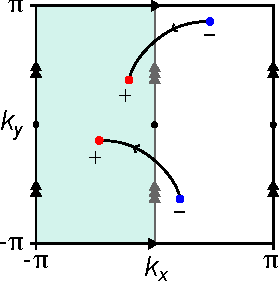
\includegraphics[width=.3\textwidth]{Images/BZ_left}}
	\caption{Top view of the 3D Brillouin torus (or 2D surface torus) for a given Weyl semimetal state obeying the glide symmetry in Equation~\eqref{eq:3D_glide}, with Weyl points and oriented Dirac strings (Fermi arcs) drawn in. Different parametrisations of the fundamental domain are shaded in teal: (a) the domain outlined in Ref.\ \cite{Fonseca-Vaidya_nonorientable}; (b) the same domain shifted in the $k_y$ direction; (c) a domain spanning the $k_y$ direction. Each of these domains is homeomorphic to $K^2\times S^1$ ($K^2$) under the boundary identifications shown. Note that the relative chirality of the two Weyl nodes in the fundamental domain changes under both alternative parametrisations.}
	\label{fig:BZ_param}
\end{figure}
For any given set of distinct Weyl points obeying the symmetry, it is possible in principle to achieve any relative chirality by reparametrising the fundamental domain. \red{This may mean that the charge of the Weyl points is fundamentally an $\N$ invariant on $K^2\times S^1$, but this is not clearly reflected in the cohomology description.} It should be noted that there do exist two planes that are of special significance, namely the so-called \emph{glide planes} at $k_x = 0$ and $k_x = \pm\pi$; these planes are (taken as a whole) invariant under the symmetry, and as such they cannot be excluded completely from any given parametrisation.

A similar point of confusion arises in explaining how the usual relation between Nielsen--Ninomiya and the Poincaré--Hopf theorem for vector fields breaks down. On the regular Brillouin torus, the factor $\h(\k)$ in the Bloch Hamiltonian can be considered a continuous vector field tangent to the torus. The Poincaré--Hopf theorem then tells us that the zeroes of such vector fields must have topological indices (corresponding to Weyl point chiralities) adding up to zero.

In the supplement to Ref.\ \cite{Fonseca-Vaidya_nonorientable}, the failure of Poincaré--Hopf is attributed to a discontinuity of the vector field at the planes $k_y=\pm\pi$ and $k_y=0$, see Figure~\ref{fig:Klein-discontinuity}.
\begin{figure}[htb!]
	\centering
	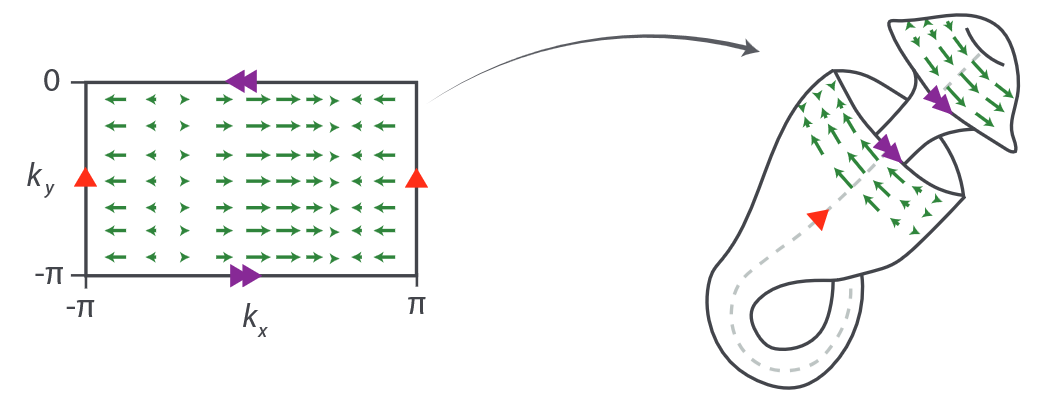
\includegraphics[width=.8\linewidth]{Images/Klein-discontinuity}
	\caption{Figure~from the supplement to Ref.\ \cite{Fonseca-Vaidya_nonorientable}. The $k_x$ component of an example $\h(\k)$ is mapped onto a $K^2$ slice of the fundamental Brillouin zone and then ``bent into shape'' to demonstrate discontinuity.
	}
	\label{fig:Klein-discontinuity}
\end{figure}
However, this mischaracterises the situation somewhat; in reality, $\h(\k)$ cannot be considered a well defined tangent vector field to $K^2\times S^1$ to begin with. This is illustrated in Figure~\ref{fig:BZ_vectors}: two vectors which point away from each other in the fundamental domain may instead point towards each other after applying the glide symmetry.
\begin{figure}[htb!]
	\centering
	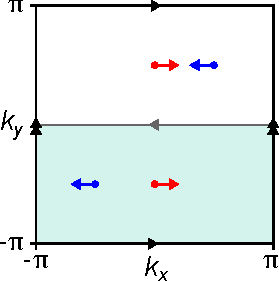
\includegraphics[width=.3\linewidth]{Images/BZ_vectors}
	\caption{Example vectors $\h(\k)$ on the glide symmetric Brillouin zone. Similar colours indicate that the vectors are related by glide symmetry.}
	\label{fig:BZ_vectors}
\end{figure}
As such, $\h$ should be thought of as a more abstract map $K^2\times S^1\to\R^3$ rather than a tangent vector field, and Poincaré--Hopf does not apply to such maps.\footnote{
	To be precise, $\h$ is a section of the trivial $\R^3$-bundle over $K^2\times S^1$, not of its tangent bundle. In the usual case of the torus, these descriptions are equivalent: $\T^3$ is parallelisable, i.e.\ $T\T^3\cong \T^3\times\R^3$. This is what allows Poincaré--Hopf to apply.}
{\color{red}
\st{In theory, one could construct a Hamiltonian starting from a proper tangent vector field to $K^2\times S^1$; this requires using gamma matrices that ``twist along'' with the tangent bundle of the manifold instead of the regular vector of Pauli matrices.}\footnote{\color{red}
	The proper construction is that of a Clifford algebra bundle over the tangent bundle, see Section 4.2 of Ref.\ \cite{Mathai_math-review}.}
[This may rely on the existence of a spin$^c$ structure, which probably does not exist in this case. This might also have implications for how ``physical'' a non-orientable BZ really is.]
}

A final point that merits clarification is the inclusion of a second glide symmetry. The supplement to Ref.\ \cite{Fonseca-Vaidya_nonorientable} discusses imposing Equation~\eqref{eq:3D_glide} together with a similar symmetry along the glide plane $k_y = 0$:
\begin{equation}
	H(k_x, k_y, k_z) = H(k_x + \pi, -k_y, k_z).
\end{equation}
It is claimed that this double symmetry subdivides the 3-torus into four copies of a different non-orientable manifold: namely $\RP^2\times S^1$, where $\RP^2$ is the real projective plane. This is broadly true, but it overlooks a seemingly innocuous detail: while the two glide symmetries have a free $\Z_2$ action on the torus individually, the action of the combined $\Z_2\oplus\Z_2$ symmetry group is no longer free. To be precise, there are four lines of high-symmetry points in the torus that are fixed by the diagonal subgroup of $\Z_2\oplus\Z_2$, similar to the time reversal invariant momenta discussed in Section \ref{sec:T-WSMs}; see Figure~\ref{fig:RP2-corners}.
\begin{figure}[htb!]
	\centering
	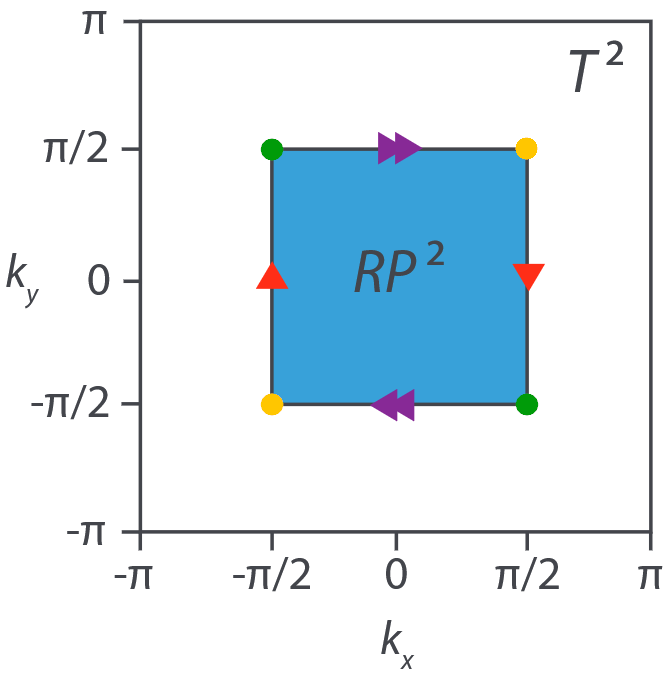
\includegraphics[width=.5\linewidth]{Images/RP2-corners}
	\caption{Figure~adapted from the supplement to Ref.\ \cite{Fonseca-Vaidya_nonorientable}. High-symmetry points (orange, green) exist for $k_x,k_y\in\{-\pi/2,\pi/2\}$; these points are fixed under simultaneous application of both glide symmetries. Similarly coloured points are related by a single glide symmetry and so they are identified on $\RP^2$.}
	\label{fig:RP2-corners}
\end{figure}
As a result, a Weyl point existing on one of these lines must have an even chirality, and it only has one symmetric partner in the 3-torus rather than the three one would expect from four identical copies of $\RP^2\times S^1$.\footnote{
	One can also argue that this must be the case topologically: if a manifold $M$ has an $n$-sheeted cover $\tilde{M}$, then the Euler characteristics of both spaces must be related by $\chi(\tilde{M}) = n\chi(M)$. Going to two dimensions, we find $\chi(\T^2) = 0$ and $\chi(\RP^2) = 1$, so that the former cannot cover the latter. Instead, the only possible covering space for $\RP^2$ is the double cover $S^2\to\RP^2$, since $\chi(S^2) = 2$.}
Such Weyl points are physically fine-tuned and are expected to split into pairs under perturbations. Nevertheless, additional symmetries may exist which force Weyl points to exist on these lines, in which case the exceptional behaviour becomes fundamental to the description. %TODO citation/remove?
Moreover, the notion of a fundamental Brillouin zone is predicated on a free group action in the main text of Ref. \cite{Fonseca-Vaidya_nonorientable}. As such, analysis of a purely $\RP^2\times S^1$ Brillouin zone cannot a priori be expected to provide the correct classification for this double glide symmetry. Indeed, similar to the case of time reversal in Section \ref{sec:T-WSMs}, a proper classification scheme should involve equivariant cohomology on the torus, bearing in mind the topological role of the high-symmetry points.\footnote{
	The mathematical description may be further complicated by the fact that the high-symmetry points are fixed only by a proper subgroup of the symmetry group. Beyond equivariant cohomology, it may be necessary to treat $\RP^2\times S^1$ as an \emph{orbifold} rather than a manifold, i.e.\ a space that encodes data about orbits of a group action. For example, the Euler characteristic of $\RP^2$ is zero as an orbifold. These spaces can be analysed using the highly specialised tool of \emph{orbifold cohomology}. \red{[On closer inspection, I'm not sure this is strictly true---most versions of orbifold cohomology seem to be an equivalent to (but perhaps more natural in this setting than) some equivariant cohomology.]}} %TODO citation
This analysis is somewhat beyond the scope of the present text, and in what follows we will restrict our attention to the case of a single glide symmetry.

\subsection{Classification scheme}

There are two main conceptual challenges that present themselves in attempting to apply consistent cohomology and homology frameworks to non-orientable systems, and in particular in developing a physical intuition for them. First of all, the analogy between second cohomology classes and Berry curvature $\Fc$ breaks down in this case, and a statement like Equation~\eqref{eq:2nd-cohom-t3} can no longer be taken to hold directly. %TODO clarify?
This is because differential forms like $\Fc$ cannot be integrated over non-orientable manifolds, and the associated (de Rham) cohomology group is actually real-valued---it cannot readily encode the $\Z_2$ invariants induced by changes in orientation. As an example, suppose we are trying to find an invariant for the 2D Klein bottle insulator obeying Equation~\eqref{eq:2D_glide}. Integrating a Berry curvature on $K^2$ directly is not well defined, while integrating over the entire Brillouin torus always yields zero: the integration is over two oppositely oriented areas. The correct $\Z_2$ invariant can be interpreted as integration with different signs on both halves of the torus, bearing in mind that the result is only gauge invariant mod 2. In order to capture this behaviour generally, we need to move to the richer but more abstract integer-valued cohomology. %TODO refer to appendix?

The second obstacle is that Poincaré duality is altered in this context. In Section \ref{sec:semimetal-topology} this form of duality was used to identify the familiar cohomology invariants with homology invariants, in the form of non-trivial oriented loops and Dirac strings. In a non-orientable system, this identification cannot be made directly; in this case, either the homology or the cohomology must be \emph{twisted} by the introduction of a \emph{local coefficient system} $\ext{\Z}$ \cites{Whitehead_Homotopy}{Hatcher_algebraic-topology}. Such a coefficient system compensates for the twist in orientation by tracking sign changes across the manifold. Introducing local coefficients on an $n$-manifold $M$ gives rise to the twisted homology and cohomology groups $H_k(M;\ext{\Z})$ and $H^k(M;\ext{\Z})$. Poincaré duality then takes the following forms \parencite[Thm. 3H.6]{Hatcher_algebraic-topology}:
\begin{align*}
	H_k(M;\ext{\Z}) &\cong H^{n-k}(M), \\
	H^k(M;\ext{\Z}) &\cong H_{n-k}(M).
\end{align*}
That is, twisting either one of the homology or cohomology restores Poincaré duality; if the homology is twisted, ordinary cohomology must be used and vice versa. When $M$ is orientable, the local coefficients become trivial and the original form of Poincaré duality is recovered from both relations.

Given the fact that Poincaré duality can be restored by twisting either the homology or the cohomology group, the correct classification of a non-orientable physical system hinges on making the correct choice between the two. Fortunately, there is a straightforward way to decide between the two in the case of a Weyl semimetal with an orientation-reversing $\Z_2$ symmetry. In this case, Poincaré duality is necessary in order to relate the chirality of Weyl points (which are cohomology invariants) to the orientation of their corresponding Dirac strings (which are the dual homology invariants). Under the orientation-reversing symmetry, Poincaré duality breaking manifests itself in the fact that the Weyl point chiralities are naturally reversed, while the orientation of Dirac strings is unchanged. This is illustrated schematically in Figure~\ref{fig:local_coefficients}.
\begin{figure}[htb!]
	\centering
	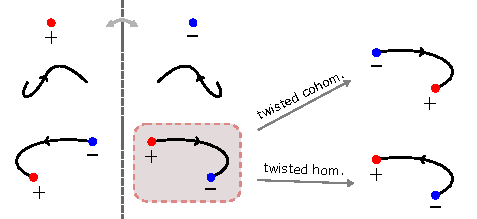
\includegraphics[width=.9\linewidth]{Images/local_coefficients}
	\caption{On the left, the action of an orientation-reversing symmetry (represented by the dashed mirror axis) is shown on a Weyl point [whose chirality is an invariant in $H^2(M\setminus W)$] and a Dirac string  [representing an invariant in $H_1(M,W)$]. The Weyl point has its chirality reversed, since the Chern number is a pseudoscalar; on the other hand, the Dirac string is mirrored but maintains its internal orientation. As a result, if the symmetry acts on a set of two Weyl points connected by a Dirac string, the resulting structure has a Dirac string whose orientation is inconsistent with the chirality of the Weyl points (shown in the shaded area)---this is a result of Poincaré duality breaking. This problem can be resolved in one of two ways: either the cohomology is twisted into $H^2(M\setminus W;\ext{\Z})$ to undo the chirality reversal, or the homology is twisted into $H_1(M,W;\ext{\Z})$ to reverse the Dirac string's orientation. Poincaré duality is restored in both cases; the correct approach depends on the physical setup.}
	\label{fig:local_coefficients}
\end{figure}
The decision of which group must be twisted can thus be made by noting how the chirality of Weyl points (outside of high-symmetry points) relates to that of their symmetric partners in the full Brillouin torus. To be precise, the presence of same-chirality pairs indicates that the (cohomological) Chern number is not reversed as expected, and the cohomology must be twisted. Meanwhile, pairs with opposite chiralities indicate that the cohomology behaves naturally, and the homology (i.e.\ the Dirac string orientations) must be twisted to follow suit.

As an example, we may apply this line of reasoning to the time reversal invariant Weyl semimetal from Section \ref{sec:T-WSMs}. This system is not usually thought of in terms of non-orientability, but the time reversal symmetry acts in an orientation-reversing way: an odd number (i.e.\ all three) of momentum directions is inverted, leading to a change of parity. Figure~\ref{subfig:TRS_orientation} illustrates that the effective Brillouin zone is indeed non-orientable.
\begin{figure}[htb!]
	\centering
	\subcaptionbox{\label{subfig:TRS_orientation}}{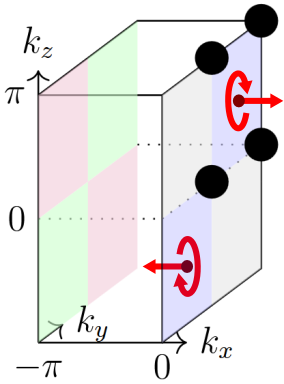
\includegraphics[width=.4\textwidth]{Images/TRS_EBZ_orientation}}
	\hfil
	\subcaptionbox{\label{subfig:TRS_Kramers}}{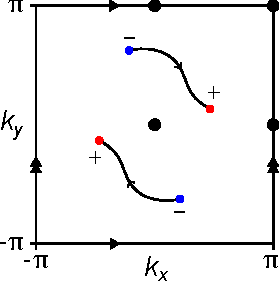
\includegraphics[width=.5\textwidth]{Images/Kramers_pairs}}
	\caption{(a) Figure~adapted from Ref.\ \cite{Thiang_equivariant}. The effective Brillouin zone under time reversal symmetry is half of $\T^3$, with additional identifications of the coloured areas as $k\sim -k$. The resulting space is non-orientable: a ``test particle'' with a given helicity is shown travelling out through the boundary at $\k = (0,\pi/2,\pi/2)\tran$, and reappearing at $\k = (0,-\pi/2,-\pi/2)\tran$ with the opposite helicity. (b) Top view of a time reversal invariant Weyl semimetal, featuring same-chirality Kramers pairs at conjugate momenta, indicating a twist in the cohomology. On the other hand, the orientation of Dirac strings is maintained by the symmetry, indicating ordinary (``untwisted'') homology.}
	\label{fig:TRS_twist}
\end{figure}
As discussed before, such systems feature Kramers pairs of Weyl points at opposite momenta related by $\k\leftrightarrow -\k$, both of which always have the same chirality; see Figure~\ref{subfig:TRS_Kramers}.
Again, these same-chirality pairs are an indication that the Chern numbers of Weyl points do not transform as expected, and so the cohomology must be twisted. It follows that the homology should not be twisted; this can also be seen directly from the fact that the Dirac strings in Figure~\ref{subfig:TRS_Kramers} have the same relative orientation. This description in terms of twisted cohomology and ordinary homology agrees exactly with the one given in Section \ref{sec:T-WSMs}, which was derived from more abstract vector bundle classification arguments in Ref.\ \cite{Thiang_equivariant}. In this particular case, direct calculation of the (co)homology groups on the effective Brillouin zone is complicated by the existence of high-symmetry points (i.e.\ the action of the symmetry is not free), which is why the authors of Ref.\ \cite{Thiang_equivariant} elect to use equivariant (co)homology on the full torus.

Returning to the case of a momentum-space glide symmetry, we can see from Figure~\ref{subfig:BZ_basic} that the situation is different here. Every Weyl point in the fundamental domain is related by symmetry to an oppositely charged point in the other half of the torus, while the orientation of Dirac strings is reversed under the symmetry. It follows that the classification of topological phases should rely on twisted \emph{homology}, and equivalently, ordinary cohomology. Since there is a proper fundamental domain in this case, there is no need to compute equivariant (co)homology groups, and we may instead rely on ordinary cohomology and twisted homology on $K^2\times S^1$.\footnote{\label{ft:eq_cohom}
	Formally speaking, equivariant cohomology of a space $M$ with a free action of the group $G$ is equivalent to ordinary cohomology on the quotient space $M/G$ \parencite[Cor. 9.6]{Tu_equivariant}.}

The choice of ordinary cohomology can be corroborated in two important ways. Firstly, the use of ordinary second cohomology classes indicates that we are classifying complex line bundles over the fundamental domain. An important insight from K-theory tells us that this is equivalent to classifying equivariant line bundles over the full torus \parencite[Prop. 2.1]{Segal_K-theory}.\footnote{
	This is related to footnote \ref{ft:eq_cohom} in the sense that K-theory is a \emph{generalised cohomology} theory.}
That is, we are classifying states that respect the symmetry directly. Secondly, the $\Z_2$ invariant found in Ref.\ \cite{Fonseca-Vaidya_nonorientable} on $K^2$-like slices of constant $k_z$ is recovered using ordinary cohomology, related to the fact that $H^2(K^2)\cong\Z_2$. Twisted cohomology would give a $H^2(K^2;\ext{\Z})\cong\Z$ invariant on these slices.

All in all, we find that the correct classification of semimetal phases in this system is given by the following Mayer--Vietoris sequence of cohomology groups on $M := K^2\times S^1$:
\begin{equation}\label{eq:MV-nonorientable}
	0 \to H^2(M) \to H^2\big(M\setminus W\big) \to H^2\left(\bigcup_{i=1}^k S_{w_i}^2\right) \to H^3(M) \to 0,
\end{equation}
where $S_{w_i}^2$ is a 2-sphere surrounding the Weyl point $w_i\in W$ as before. Equivalently, the classification may be given in terms of the following dual \emph{twisted} homology sequence:
\begin{equation}\label{eq:homology-sequence-nonorientable}
	0 \to H_1(M;\ext{\Z}) \to H_1\big(M, W;\ext{\Z}\big) \overset{\partial}{\to} H_0(W;\ext{\Z}) \to H_0(M;\ext{\Z}) \to 0.
\end{equation}
In what follows, we will provide explicit computations of these groups and discuss the associated invariants.


\subsection{Computing invariants}

The use of ordinary cohomology groups in the Mayer--Vietoris sequence \eqref{eq:MV-nonorientable} means calculations are relatively straightforward, and standard techniques such as cellular cohomology can be applied. \red{[Should I make a small Appendix B containing an example cellular cohomology calculation?]} Using these methods, we calculate the sequence to be
\begin{equation*}
	0\to \mathbb{Z}\oplus\mathbb{Z}_2 \to \mathbb{Z}^{1+k}\oplus\mathbb{Z}_2 \to \mathbb{Z}^k \to \mathbb{Z}_2 \to 0.
\end{equation*}

%TODO

{\color{blue}
\begin{itemize}	
	\item Cohomology is easy to compute, but its dual twisted homology offers a very intuitive perspective of the invariants, demonstrating how the $\Z^3$ invariant on a 3D Chern insulator gets reduced to a $\Z\oplus\Z_2$ under this symmetry. The $\Z_2$ factor is precisely the $\Z_2$ invariant discussed by Fonseca, Vaidya et al. This intuition is especially clear when viewed as twisted equivariant homology on $\T^3$. [Include pictures of the action of the symmetry on the three basic homology invariants on $\T^3$.]
	
	\item Under this description, the semimetal Mayer--Vietoris sequence becomes
	\begin{equation*}
		0\to H^2(K^2\times S^1) \to H^2(K^2\times S^1\setminus W) \to H^2(S_W) \to H^3(M) \to 0,
	\end{equation*}
	which can be calculated explicitly (using e.g. cellular (co)homology) as
	\begin{equation*}
		0\to \mathbb{Z}\oplus\mathbb{Z}_2 \to \mathbb{Z}^{1+k}\oplus\mathbb{Z}_2 \to \mathbb{Z}^k \to \mathbb{Z}_2 \to 0.
	\end{equation*}
	From the $\Z_2$ in the last term, we immediately recover the $\Z_2$ charge cancellation no-go theorem. It also becomes clear that a single Weyl point may carry non-trivial topology (i.e. already adds a factor to the group of invariants).
\end{itemize}

Additionally:

\begin{itemize}
	\item The description can easily be extended to a 2D type AIII Klein bottle WSM with chiral symmetry; in this case, 1st cohomology invariants (winding numbers) are dual to twisted 1st homology invariants (Fermi arcs/loops).
	
	\item More elementary systems such as 3D type A with inversion symmetry also exhibit non-orientable EBZs, but in this case the description is complicated by the existence of fixed points (the TRIM).
	
	\item Applicability of this description is probably limited under addition of non-trivial additional bands, e.g. 4-band models incorporating spin and orbital degrees of freedom. The full scope of applicability is somewhat of an open question at this point. (E.g., how well are 2D chiral WSMs described by this homology picture?)
\end{itemize}
}



{\color{red}
\section*{Notes}
Concepts explored in early personal notes:
\begin{itemize}
	\item Calculations of (co)homology and semimetal MV sequence for manifolds in $\geq2$ dimensions:
	\begin{itemize}
		\item All compact surfaces without boundary, i.e.\ the surfaces $M_g$ and $N_g$
		
		\item All spaces of the form $M = K^2 \times \T^{d-2}$
	\end{itemize}
	
	\item The map $\Sigma:H^{d-1}(\bigsqcup_{k}S^{d-1})\to H^d(M)$ in the semimetal MV has a clear interpretation in terms of total charge in the (orientable) $d=3$ case. This would provide a clear picture of the total charge cancellation in the orientable case ($H^d(M) = \Z$ in general) vs. the mod 2 charge cancellation in the non-orientable case ($H^d(M) = \Z_2$ in general).
	
	\item However, $\Sigma$ and the other maps in the MV sequence are difficult to interpret in the $\chi\neq 0$ case (maybe even generally for odd dimensions). Taking the oriented case as an example, the MV sequence ends as
	\begin{align*}
		H^{d-1}(M\setminus\Delta)\ \rightarrow\ H^{d-1}\left(\bigsqcup_{k}S^{d-1}\right) \cong \Z^k\ \overset{\Sigma}{\rightarrow}\ H^d(M) \cong \Z
	\end{align*}
	so that the ``charge configuration'' in $\Z^k$ must map to 0 by $\Sigma$ in order to descend from the semimetal, regardless of whether $\chi=0$.
	
	\item This may imply that the Bloch vector field carries more topological information about the total charge than the MV sequence (which makes sense since it generates \emph{all} homology groups of the valence bundle, and all Betti numbers factor into $\chi$). As a concrete example, consider $M=S^2$ with a single puncture of charge $+2$. The punctured sphere is topologically a disc, so that the valence bundle must be trivial, while the Bloch vector field is topologically non-trivial in the sense that it has an index $+2$ singularity. In addition, all relevant $H_n(A)\oplus H_n(B)$ are zero, so that the semimetal MV reduces to the statement that $H_2(S^2)\cong H_1(S^1)$.
	
	\item It may even be the case that the valence bundle cannot be generated from the Bloch vector field in the $d=2$ case; it's probably worth studying the $d\in\set{3,4,5}$ cases (pullback of some universal bundle) to learn more about this. The $d=3$ case should be especially helpful in understanding how the valence bundle arises from the vector field.
	
	\item A complicating factor in the non-orientable case is that the homology groups are different from the cohomology groups, since the torsion moves up one dimension. This makes the homological semimetal MV different from the cohomological one (it's a short exact sequence in $d\geq3$!), and this leads to additional challenges in interpretation.
	
	\item The map $H: \R^3\to\la[su](2),\ \vec{h}\mapsto \vec{h}\cdot\vec{\sigma}$ is an isomorphism of Lie algebras, with the cross product as a Lie bracket on $\R^3$. Still the vector field is discontinuous on a non-orientable manifold, while $H$ is not. This suggests an alternative approach for constructing the valence bundle: consider $h$ as a map $M\to\R^d$ instead of an element of $\vct(M)$, and then pull back the universal bundle along the unit map $\hat{h}:M\setminus\Delta\to S^{d-1}$. That is, we detach $\vec{h}$ from the tangent bundle and consider it a more abstract map. An added ``benefit'' of this is that we lose all coordinate dependence. However, this may also be a downside in the sense that the map will not be subject to the same constraints (Poincaré--Hopf etc.) that the vector field is; for example, $S^2\to\R^2,\ x\mapsto(1,0)$ is a perfectly valid map that would violate the hairy ball theorem as a vector field (and this is a result of being unable to cover $S^2$ by a single chart). At this point the question may become more about which description is more physical in nature, and the non-orientable Weyl point paper\cite{Fonseca-Vaidya_nonorientable} seems to imply there may be more to the $h:M\to\R^3$ story. It also seems to agree better with the intuition of an applied external potential removing all Weyl nodes -- something that's impossible for $\chi\neq0$ if charge corresponds to vector field index. It also explains how the valence bundle can be trivial on the once punctured $S^2$.
	
	\item In light of the previous point, this may be an important observation: every $d$-manifold $M$ with $\chi(M)=0$ admits a nowhere-vanishing vector field (\href{https://math.stackexchange.com/questions/47370/if-a-manifold-m-has-zero-euler-characteristic-there-is-a-non-vanishing-vector-f}{link}). \st{This may imply that the vector field description is equivalent to the map to $\R^d$ in these cases, though one needs to be careful about charts. It would be good to find or write a (dis)proof for something like $\vct(M)\cong\Cinf(M,\R^d)$ (or similar for non-vanishing maps) in this case. Or more specifically:}
	\[
		\st{\big[M\setminus\Delta,S^{d-1}\big] \stackrel{?}{\cong} \Set{\vec{h}\in\vct(M\setminus\Delta) | \text{$\vec{h}$ is non-vanishing}}}
	\]
	Update: I think the real requirement for equivalence is that the base manifold $M$ is parallelisable (i.e.\ has a trivial tangent bundle), since we're essentially using a trivial $\R^d$-bundle in this construction.
	
	\item Any smooth $d$-manifold can be given a CW complex structure with one $d$-cell (\href{https://mathoverflow.net/questions/120799/manifolds-admitting-cw-structure-with-single-n-cell}{link}). On this $d$-cell there is an exact correspondence between vector fields and maps to $\R^d$, since it can be embedded in $\R^d$. What distinguishes the two is how points on the boundary of the $d$-cell are identified with each other; this determines whether the ``vectors'' need to change orientation. To illustrate:
	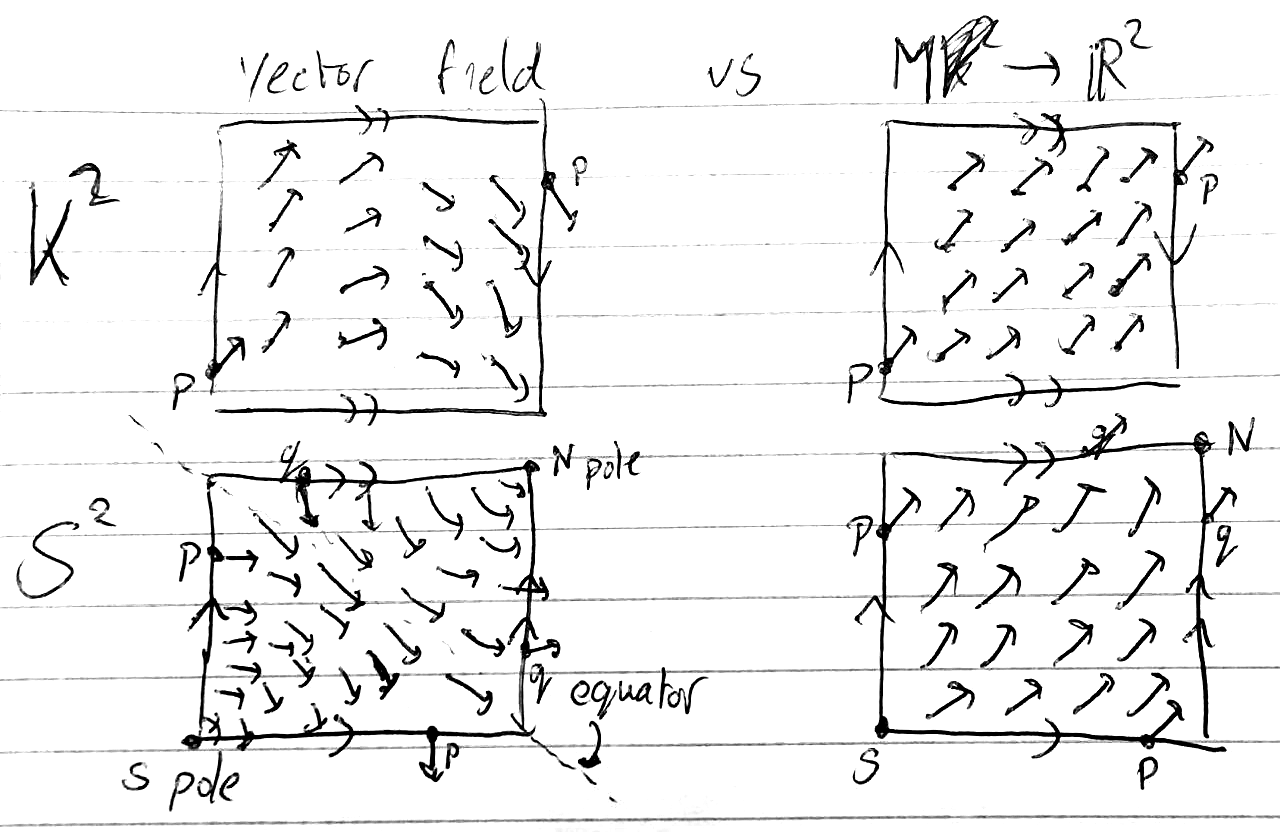
\includegraphics[width=.9\textwidth]{Images/vectorfield-vs-map}
	
	\item On any orientable manifold, the Stokes' theorem argument shows that the total charge must be zero regardless of Euler characteristic:
	\[
		\sum_{\alpha}w(S_\alpha) = \sum_{\alpha}\int_{S_\alpha} c_1(E) = \sum_{\alpha}\int_{S_\alpha}\frac{\Tr\Fc}{2\pi} = \int_{B'} \dd{\frac{\Tr\Fc}{2\pi}} = 0
	\]
	where the last equality holds by the Bianchi identity for the trace. This means the valence bundle cannot be a pullback along a tangent vector field for $\chi\neq0$.
	
	On a non-orientable manifold, this argument doesn't hold since the integral over $B'$ isn't well defined.
	
	\item Total chirality isn't well defined on a non-orientable manifold (at least in odd dimensions, not sure how to interpret even dimensions). Still there is charge cancellation in the form of Fermi arcs etc.; it may take moving to a different homology system to get the full picture, such as homology with local coefficients or equivariant homology. (See e.g. \cite{Thiang_equivariant})
	
	\item It may be worth classifying which manifolds are candidates for physical material Brillouin zones; I have a feeling that this might be restricted to those manifolds for which the $n$-torus is a covering space. In this case a full classification of symmetries on the torus (and e.g. their related equivariant homologies) would be sufficient to classify all material topologies. This classification is related to space group symmetries.
\end{itemize}
}  % end red colour

\appendix 

\cftaddtitleline{toc}{chapter}{$\qquad$APPENDICES}{}
\chapter{Homology and cohomology}

The concepts of homology and its counterpart cohomology are indispensable in algebraic topology. \red{[\ldots]}  %TODO

Here we offer a brief introduction to these concepts, aimed at the uninitiated physicist. The goal here is not to be completely rigorous, but to give a sufficiently complete understanding that the applications discussed in the main text may be understood in their proper context. For a more complete picture, the interested reader is referred to standard texts in algebraic topology such as \cite{Hatcher_algebraic-topology} and \cite{Bredon_topo-geometry}. A more geometric treatment is also found in \cite{Bott-Tu_differential-forms}.


\section{Homology}

Suppose we have some topological space---for example, the torus $\T^2$---and we want to study \red{[\ldots]}%TODO

The basic idea underlying homology is that information about the topology of a space can be gained from studying non-trivial subspaces. In the related \emph{homotopy} theory, this is achieved by mapping $n$-dimensional spheres into the space; if the image of such a map cannot be contracted to a point, the map represents a non-zero element of a homotopy group.


\section{Cohomology}

\printbibliography

	
\end{document}